\documentclass[lof,lot,12pt,progress]{puseniorthesis}
%options to class:
% lof - generate list of figures
% lot - generate list of tables
% Xpt - font size
% filecopy - note that this is 'File Copy' on title page
% advisercopy - note that this is 'Adviser Copy' on title page
% readercopy - note that this is 'Reader Copy' on title page
% progress - change title page to say 'Progress Report' instead of 'Final Report'

%%%%%%%%%%%%%%%%%%%%%%%%%%%%%%%%%%%%%%%%%%%%%%%%%%%%%%%%%%%%%%%
% START CUSTOM INCLUDES & DEFINITIONS
%%%%%%%%%%%%%%%%%%%%%%%%%%%%%%%%%%%%%%%%%%%%%%%%%%%%%%%%%%%%%%%

%-------------------------------------------------------------
% 1. CORE MATH & FONT PACKAGES
%-------------------------------------------------------------
\usepackage{amsmath,amssymb,amsfonts, amsthm}
\usepackage{mathtools}
\usepackage{mymath}
\usepackage{MnSymbol}

%-------------------------------------------------------------
% 2. REFERENCE & HYPERLINKING
%-------------------------------------------------------------
\usepackage[hidelinks]{hyperref}
\hypersetup{draft=false}

\usepackage[backend=bibtex, sorting=none, firstinits=true, abbreviate=true, url=false, isbn=false]{biblatex}
\addbibresource{references.bib}

%-------------------------------------------------------------
% 3. FIGURES, GRAPHS, & DRAWING (TikZ/PGF)
%-------------------------------------------------------------
\usepackage{tikz}
\usepackage{pgfplots}
\pgfplotsset{compat=newest}
\usetikzlibrary{plotmarks}
\usepgfplotslibrary{groupplots}

\usetikzlibrary{shapes, arrows, shapes.misc, arrows.meta, positioning, matrix, calc, fit, fadings, patterns}
\usetikzlibrary{calc,patterns,decorations.pathmorphing,decorations.markings,arrows, arrows.meta}
\usepackage{varwidth}
\usepackage[export]{adjustbox}
\usepackage{overpic}

%-------------------------------------------------------------
% 4. FLOATING OBJECTS, CAPTIONS, & LAYOUT
%-------------------------------------------------------------
\usepackage{caption}
\usepackage{subcaption}
\usepackage{placeins}

% That's because it likes placing large figures on their own page even though there's space for text
\renewcommand{\floatpagefraction}{0.7}
\renewcommand{\textfraction}{0.1}
\renewcommand{\topfraction}{0.9}
\renewcommand{\bottomfraction}{0.9}

%-------------------------------------------------------------
% 5. TABLES & ALIGNMENT
%-------------------------------------------------------------
\usepackage{arydshln}
\usepackage{tabto}
\usepackage{siunitx}
\usepackage{nth}

%-------------------------------------------------------------
% 6. ALGORITHMS & PSEUDOCODE
%-------------------------------------------------------------
\usepackage{algorithm}
\usepackage[noend]{algpseudocode}
\usepackage{xcolor}

\definecolor{commentgrey}{gray}{0.6}
% This ensures lines with comments do not shrink
\newcommand{\algcomment}[1]{%
  \hfill\mbox{}\Comment{\textcolor{commentgrey}{#1}}%
}
% OLD COMMAND
% \newcommand{\algcomment}[1]{\scriptsize\textcolor{commentgrey}{\Comment{#1}}}

%-------------------------------------------------------------
% 7. THEOREM-LIKE ENVIRONMENTS
%-------------------------------------------------------------
\newtheorem{theorem}{Theorem}[section]
\newtheorem{corollary}[theorem]{Corollary}
\theoremstyle{definition}
\newtheorem{definition}[theorem]{Definition}
% \newtheorem{assumption}{Assumption}
% \newtheorem{remark}{Remark}

%-------------------------------------------------------------
% 8. UTILITY & CLASS FILE MODIFICATIONS
%-------------------------------------------------------------
\usepackage{todonotes}

%-------------------------------------------------------------
% 9. CUSTOM MATH OPERATORS & COMMANDS
%-------------------------------------------------------------
\newcommand{\Argmin}{\ensuremath{\mathop{\mathrm{argmin}}}}
\newcommand{\Argmax}{\ensuremath{\mathop{\mathrm{argmax}}}}
\newcommand{\twonorm}[1]{\left\| #1 \right\|_2}
\newcommand{\set}[2]{\left\{ #1 \;\middle|\; #2 \right\}}
\newcommand{\Rset}{\mathcal{R}}
\newcommand{\inR}[3]{#1 \in \Rset^{#2 \times #3}}
\newcommand{\trans}[1]{#1^\top} % we do not use this, ^T instead

%%%%%%%%%%%%%%%%%%%%%%%%%%%%%%%%%%%%%%%%%%%%%%%%%%%%%%%%%%%%%%%
% END CUSTOM INCLUDES & DEFINITIONS
%%%%%%%%%%%%%%%%%%%%%%%%%%%%%%%%%%%%%%%%%%%%%%%%%%%%%%%%%%%%%%%

% Required inputs:
\author{Claudio Vestini}
\classyear{`26}
\adviser{Ryne Beeson, \newline Bartolomeo Stellato (ORFE)}
\reader{\textcolor{red}{READER}}
\title{\textcolor{red}{TITLE}}
\dept{Mechanical and Aerospace Engineering}
\submitdate{April 23, 2026}
\course{MAE 499}
\abstract{Euclidean projections onto intersections of polyhedral sets are essential operations in constrained optimisation. Dykstra's algorithm provides an efficient iterative method for computing these projections; however, its practical utility is limited by a stalling phenomenon that can result in arbitrarily long execution cycles. The primary theoretical contribution of this thesis is the formalisation of the stalling condition and the derivation of its duration in closed form. Building on this mathematical resolution, a fast-forward modification is introduced that detects stalling and advances the internal memory variables beyond the stalling cycle in a single computational step. This modification eliminates the algorithm's unpredictable execution time while preserving its asymptotic convergence guarantees.

An accelerated version of the stall-averse solver is integrated within a large-scale, inexact projected gradient descent framework to address density estimation tasks via optimal transport. Specifically, we approximate Knothe-Rosenblatt triangular maps parameterised by a probabilist's Hermite polynomial basis. Empirical estimation of these maps requires enforcing monotonicity over a discrete sample ensemble, which yields an ill-conditioned polyhedral feasible set. The modified Dykstra algorithm is consequently employed to compute the required Euclidean projections onto this geometric structure.

The combined architecture is evaluated across two nonlinear tracking domains. In astrodynamics, the framework is applied to non-Gaussian uncertainty propagation in orbital dynamics, reconstructing the physical ground-truth shears of satellite state distributions when classical filters are inadequate. In geophysical data assimilation, the engine is used with the Lorenz 1963 system to approximate continuous mappings of chaotic probability densities. These results collectively demonstrate the robustness and scalability of the framework for mapping uncertainty distributions.}

% Optional inputs (any of these can be omitted)
% \extranotes{These are a few lines of optional notes} 
\dedication{\textcolor{red}{DEDICATION}}
\acknowledgements{\textcolor{red}{AKNOWLEDGMENTS}}

\numberwithin{equation}{section}

\begin{document}

\chapter{Introduction} \label{ch:introduction}
\section{The landscape of space situational awareness}

The near-Earth space environment has experienced an unprecedented densification over the last decade. With the advent of massive satellite constellations and the compounding accumulation of orbital debris, space situational awareness has transitioned from a monitoring exercise into a critical, high-frequency computational challenge. Simultaneously, the modern geopolitical and scientific focus has rapidly expanded outwards to the cislunar domain, the vast, complex region of space encompassing the Earth, the Moon, and the Lagrange points that balance their gravitational pulls. 

Driven by international initiatives like the Artemis programme and the Lunar Gateway, the cislunar environment is slated to become the next major frontier for human presence and autonomous satellite operations. Both of these regimes demand a fundamental paradigm shift in how we track resident space objects. In near-Earth orbit, operators must rigorously track the evolution of probability density functions over time to accurately assess collision probabilities. In the cislunar environment, modelling continuous multi-body gravitational interactions results in highly non-linear dynamics where trajectories are incredibly sensitive to initial conditions.

Consequently, the deterministic tracking of satellites, representing them as single, certain points in space, is not sufficient. To maintain safe operations, prevent collisions, and ensure mission viability across all orbital regimes, astrodynamicists are transitioning from tracking singular points to propagating entire clouds of uncertainty.

\section{The breakdown of Gaussian assumptions} \label{sec:gaussian_breakdown}

The state of an object in orbit is most commonly parameterised using a set of coordinates known as the \emph{equinoctial} elements, which are six-dimensional. This coordinate system resolves the mathematical singularities inherent in classical \emph{Keplerian} elements. However, propagating probability distributions through the highly non-linear dynamics of orbital mechanics introduces significant analytical difficulties. While the initial uncertainty of a satellite's state immediately following an observation might be well-approximated by a multivariate Gaussian distribution, the true physical distribution rapidly distorts as the states are propagated forward in time. 

The primary driver of this distortion is the physical ground truth shear of the orbital environment. Differential gravitational effects, atmospheric drag, and solar radiation pressure collectively induce non-linear shearing on the state space. As the uncertainty cloud is pushed through these dynamics, it stretches, folds, and develops heavy tails, frequently exhibiting distinct ``boomerang" or highly coupled geometries~\cite{Horwood2014}.

\begin{figure}
    \centering
    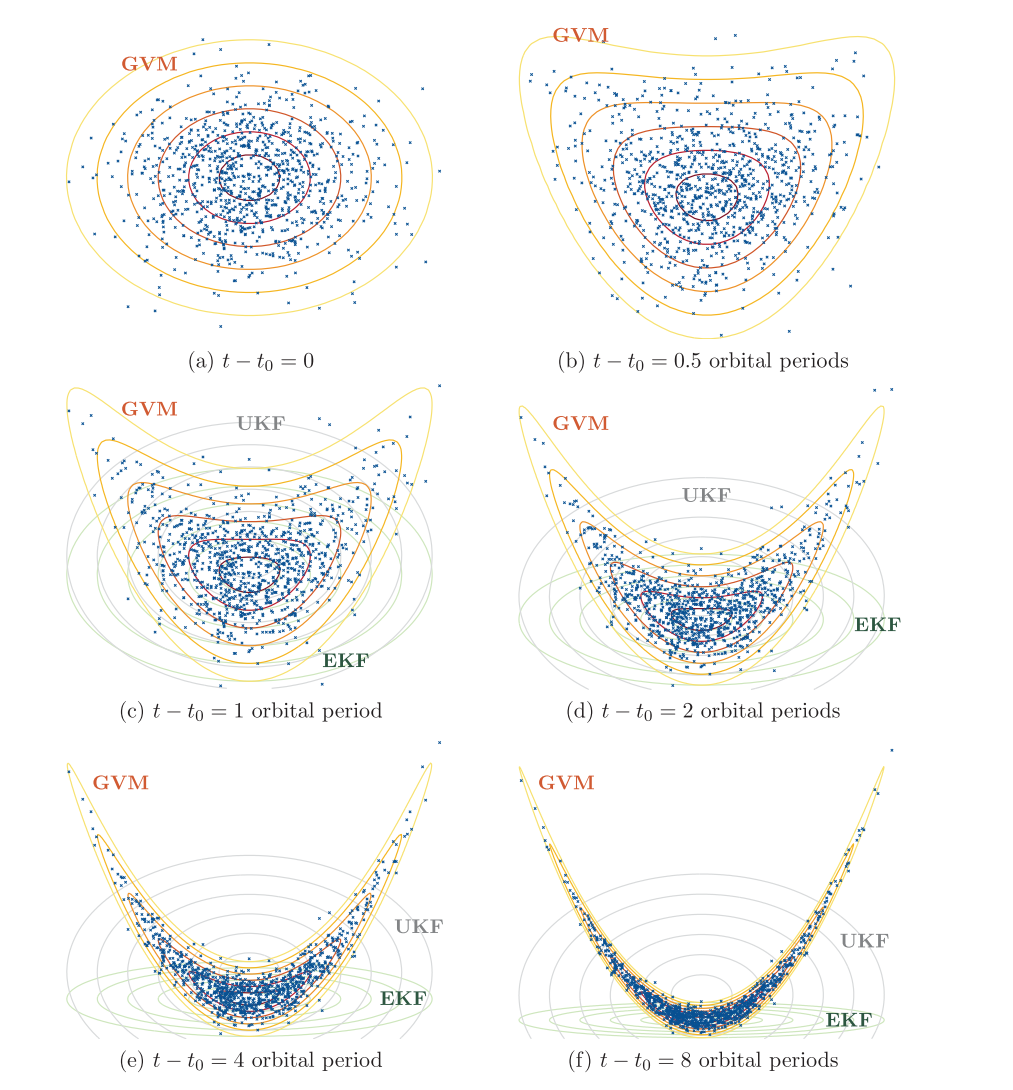
\includegraphics[width=\linewidth]{figures/Horwood_distributions.png}
    \caption{Evolution of equinoctial elements across propagation epochs~\cite{Horwood2014}.}
    \label{fig:horwood_distributions}
\end{figure}

Classical filtering techniques, such as the Extended Kalman Filter (EKF) and the Unscented Kalman Filter (UKF), are fundamentally ill-equipped to handle these dynamics over extended time horizons. These methods implicitly assume that the underlying probability distribution remains at least approximately Gaussian. Constraining the propagated uncertainty within a linearised Gaussian covariance ellipsoid fundamentally mischaracterises the underlying non-linear dynamical flow. By forcing this rigid geometry over a highly sheared physical distribution, classical filters frequently position their maximum likelihood estimate entirely outside the support of the true state~\ref{fig:horwood_distributions}. Consequently, the filter erroneously assigns peak probability density to regions of the state space where the actual physical measure is strictly zero.

This effect is visualised in Figure~\ref{fig:horwood_distributions}, where a particle cloud approximating a set of low-Earth equinoctial orbital elements is forward-propagated over several orbital periods. Three probability distributions are fitted to these data, namely two Gaussians emanating from the EKF and UKF, respectively, and a Gauss Von Mises (GVM) distribution, which more accurately models the nonlinear shearing of the orbital elements (more in Chapter~\ref{ch:experiments_and_applications}). A two-dimensional slice along the semi-major axis--mean longitude plane is then plotted alongside each of the three probability contours. From Figure~\ref{fig:horwood_distributions}, it is clear that the GVM distribution strongly outperforms the EKF and UKF over long-term propagation. This divergence between assumed mathematical models and physical reality necessitates a different approach to uncertainty modelling, one that can embrace and accurately represent arbitrary non-Gaussian distributions.

\section{Optimal transport and triangular maps}

To capture the complex, sheared distributions dictated by orbital mechanics, we turn to the mathematical theory of optimal transport. Originating from the problem of finding the most efficient way to move piles of earth to fill construction trenches~\cite{monge1781memoire}, this discipline provides a rigorous framework for defining a continuous mathematical map that pushes a simple, easy-to-sample reference distribution onto a more complex target distribution (such as that discussed in Section~\ref{sec:gaussian_breakdown}).

Instead of propagating the physical probability measure directly through the non-linear dynamical flow, optimal transport frames the uncertainty quantification problem as learning a continuous pushforward map between two distinct probability spaces. This deterministic transformation acts as a structural bridge, coupling a tractable, well-characterised reference measure, such as an isotropic standard Gaussian, directly to the highly complex, sheared target distribution dictated by the physical ground truth. By accurately reconstructing this map, we can bypass the local linearisation flaws of classical filters. We can draw vast ensembles of independent, identically distributed samples from the simple reference space, push them forward through our learned map, and thus recover the true, heavy-tailed non-Gaussian geometry of the evolved physical uncertainty cloud.

% However, discovering a general optimal transport map in a high-dimensional setting is inherently challenging; without structural restrictions, the computational cost of searching for an arbitrary mapping grows restrictively large as the state space expands. To render the problem computationally tractable, one can impose a structural constraint on the transformation by seeking a \emph{triangular map}. Instead of attempting to map the entire multi-dimensional space simultaneously, this map decomposes the problem by imposing a lower-triangular structure, dictating that each successive dimension of the state vector is constructed using only the information from the dimensions that preceded it. By mirroring the natural, step-by-step conditional dependencies of the physical system, the triangular formulation serves as an ideal framework for tracking the cascading, coupled uncertainties present in orbital mechanics.

\section{Computational challenges}

While triangular maps provide an elegant theoretical framework for probability transport, translating this continuous abstraction into a functional computational tool introduces significant engineering challenges. In learning multi-dimensional maps, first-order optimisation methods such as projected gradient descent (PGD) offer significant computational advantages over more sophisticated frameworks such as quasi-Newton or interior-point methods used in the literature~\cite{Baptista2022}.

In the PGD framework we propose in this thesis, to preserve the physical validity of the transported probability distribution, the learned map must remain strictly monotonic. This requirement manifests as a large number of linear inequality constraints, defining a strict permissible region for the map's parameters. Geometrically, this space of valid parameters forms a sparse, multi-dimensional polyhedron. Whenever the PGD algorithm pushes the parameters outside the valid region, they must be mathematically mapped back to the closest point on the boundary of the polyhedron. This fundamental operation is known as a Euclidean projection.

\section{Dykstra's algorithm and stalling}

Since we require a Euclidean projection at every single epoch of a high-frequency learning loop, the choice of projection algorithm dictates the overall viability of the tracking framework. Standard interior-point optimisation software is often computationally prohibitive for such large-scale, high-dimensional tasks. Dykstra's projection algorithm offers a computationally inexpensive, scalable solution to compute these Euclidean projections. Utilised across various engineering disciplines---such as restricted least squares in machine learning or model predictive control---Dykstra's algorithm breaks down the (often intractable) joint projection into a sequence of simple iterative steps, offering phenomenally low per-iteration computational overhead.

However, Dykstra's algorithm harbours a fatal mathematical flaw known as the stalling phenomenon. In specific geometric configurations, particularly near the sharp, complex intersections of multiple constraint planes, the iterates can be subject to arbitrarily long cycles. During these unpredictable stalling periods, the algorithm stops moving towards the true optimal projection. In safety-critical or real-time applications, where a fixed iteration budget is utilised to satisfy computational constraints (such as our optimal transport framework), the stalling phenomenon can completely inhibit the feasible deployment of Dykstra's algorithm. Furthermore, the standard ``vanilla'' implementation of this algorithm lacks any optimisation enhancement, a gap that must be closed to allow Dykstra's integration in space-ready software.

\section{Summary of contributions}

This thesis bridges the gap between fundamental algorithmic optimisation and high-dimensional physical modelling. As a cross-disciplinary effort between the Operations Research and Financial Engineering (ORFE) and the Mechanical and Aerospace Engineering (MAE) departments, the core contributions of this work are explicitly dual in nature, forming two distinct yet interconnected main sections.

First, we resolve the known stalling phenomenon in Dykstra's algorithm. By rigorously analysing the geometry of polyhedral constraints, we derive an exact, closed-form mathematical solution for the duration of the stalling period. Building upon this derivation, we introduce a fast-forward modification to the algorithm. When a stall is detected, a single, computationally inexpensive update instantly advances the internal memory variables to the end of the stall. Alongside several other optimisation enhancements, these modifications eliminate the unpredictable convergence behaviour of the algorithm while preserving its strong asymptotic convergence guarantees, transforming it into a highly robust engine for real-time and safety-critical engineering applications.

Second, we architect a scalable software framework for optimal transport in orbital mechanics. Leveraging the fast-forward modified Dykstra solver, we construct a robust PGD framework to learn triangular maps. By successfully reconstructing non-linear physical ground truth shears, we establish this combined engine as a viable, highly performant alternative to traditional filtering. Ultimately, we demonstrate that optimal transport, when coupled with rigorous mathematical optimisation, can fundamentally advance the state-of-the-art in space domain awareness. This applied framework paves the way for dynamically tracking complex, non-Gaussian uncertainty distributions across diverse orbital regimes, providing a critical computational tool for ensuring safe, reliable, and autonomous operations in the modern space environment.

\section{Thesis outline}

The remainder of this thesis is structured as follows. 

Chapter~\ref{ch:dykstra} focuses on the theoretical advancements to Dykstra's projection algorithm. It introduces the geometry of Euclidean projections and polyhedral sets, formally defines the stalling phenomenon, and presents the mathematical proof for the closed-form duration of the stall. The chapter concludes by defining the fast-forward modified algorithm and demonstrating its superiority on pathological constraint geometries.

Chapter~\ref{ch:optimal_transport} pivots to the aerospace application, formally defining the theory of optimal transport and the structure of triangular maps. It details the parameterisation of these maps and formulates the monotonicity requirements into a constrained optimisation problem.

Chapter~\ref{ch:optimisation} details the architecture of the custom Python software framework. It outlines the integration of the outer learning loop, featuring stochastic gradient descent and several other dynamic learning schedules.

Chapter~\ref{ch:experiments_and_applications} presents the empirical results of applying the framework to orbital mechanics and geophysical applications. It features the successful reconstruction of physical ground truth shears and provides performance scaling metrics demonstrating the computational efficiency of the combined architecture. 

Finally, Chapter~\ref{ch:conclusion} summarises the primary findings, details the broader implications for both the optimisation and astrodynamics communities, and proposes avenues for future theoretical and applied work.

\chapter{Fast-forwarding stalling in Dykstra's algorithm} \label{ch:dykstra}
Deploying constrained learning algorithms requires a highly efficient method for computing Euclidean projections. Dykstra's algorithm~\cite{DYKSTRA} offers a computationally lightweight solution to find the projection of an initial point onto the intersection of multiple convex sets~\cite{KEMPF20206542}. However, despite its strong theoretical guarantees, Dykstra's algorithm is mathematically encumbered by the stalling phenomenon~\cite{DYKSTRASTALLING}. Because the duration of these stalling periods is unknown \emph{a priori}, the algorithm cannot be reliably restricted to a fixed iteration budget. This unpredictable convergence behaviour inhibits the deployment of Dykstra's method in practical, real-time computational software.

In this chapter, we address the stalling problem of Dykstra's method for polyhedral sets. Exploiting simplifications that arise in the polyhedral case, we derive the exact closed-form duration of the stalling period once stalling is detected. This mathematical derivation enables a modified version of Dykstra's algorithm that instantly fast-forwards through the stalling period, thereby eliminating unpredictable computational cycles. Crucially, this modification preserves all asymptotic convergence guarantees of the original algorithm. This theoretical development forms the fundamental optimisation pillar of this thesis, transforming Dykstra's method into a robust, predictable engine ready for safety-critical engineering applications.

% The structure of this chapter is as follows. Section~\ref{sec:euclidean_projections} reviews the mathematical background of Euclidean projections and the method of alternating projections. Section~\ref{sec:dykstra_algorithm} introduces Dykstra's algorithm and its specific simplifications for polyhedral sets. Section~\ref{sec:stalling_phenomenon} formally defines the stalling phenomenon. Section~\ref{sec:closed_form_solution} presents the rigorous mathematical proof for the closed-form duration of the stall. Section~\ref{sec:fast_forward_algorithm} proposes the fast-forward algorithmic modification, and Section~\ref{sec:dykstra_numerical_experiments} presents supporting numerical experiments to demonstrate the algorithmic superiority of the proposed framework on pathological constraint geometries.

\section*{Notation}
We denote the transpose of a vector $w$ as $w^T$, and its $\ell_{2}$-norm as $\twonorm{w}$. The interior of a set $\mathcal{H}$ is denoted as $\text{int}\,\mathcal{H}$, and its boundary is denoted as $\partial\mathcal{H}$. Function composition is written as $f \circ g$, and the modulo and ceiling operators are denoted by $[\cdot]$ and $\lceil \cdot \rceil$, respectively. The absolute inner Dykstra iteration index is denoted as $m$ and raised as a bracketed superscript (e.g., $w^{(m)}$), while the outer learning iteration index is denoted as $t$. The spatial dimension of the decision variable is denoted as $d$. The individual half-space index is denoted as $i$, while the total half-space count is denoted as $n$ and remains fixed. We name an update with an increase by $1$ in $m$ ($m \leftarrow m+1$) an \emph{iteration}, and refer to an advancement of $n$ iterations ($m \leftarrow m+n$) as a \emph{cycle}.
\section{Background on Euclidean projections} \label{sec:euclidean_projections}

At the core of many problems in optimisation, statistics, and machine learning lies the task of identifying a point that satisfies multiple constraints simultaneously~\cite[Ch. 8]{BOYDCONVEX}. Formally, we consider a Euclidean space $\mathcal{X} \subseteq \Rset^p$ equipped with the Euclidean norm $\twonorm{x}\eqdef (x_1^2+\dots+x_p^2)^{1/2}$, and a finite family of $n$ closed convex subsets $\{\mathcal{H}_i\}_{i=0}^{n-1}\subseteq\mathcal{X}$ with a nonempty intersection $\mathcal{H} := \bigcap_{i=0}^{n-1} \mathcal{H}_i$. Given a point $x^\circ \in \mathcal{X}$, its Euclidean projection $x^\star \reqdef \mathcal{P}_{\mathcal{H}}(x^\circ)$ onto set $\mathcal{H}$ can be found by solving the \textit{constrained quadratic program} (CQP)
\begin{equation} \label{eq:projection}
\begin{array}{ll}
    {\displaystyle \minimise_{x\in\mathcal{X}}}  & \frac{1}{2}\twonorm{x-x^\circ}^2 \\
    \text{subject to} & x \in \bigcap_{i=0}^{n-1}\mathcal{H}_i,
\end{array}
\end{equation}
where $x$ is the decision variable, and $x^\circ$ and sets $\{\mathcal{H}_i\}_{i=0}^{n-1}$ are the problem data. In this paper, we assume $\mathcal{H}$ to be a polyhedral set, meaning $\mathcal{H}=\set{x \in \mathcal{X}}{A x \leq b}$, with $A \in \Rset^{n\times p}$ and $b \in \Rset^n$, and each $\mathcal{H}_i$ a half-space, written as
\begin{align}\label{eq:sets_i}
\mathcal{H}_i\coloneqq\set{x\in\mathcal{X}}{a_i^Tx \leq b_i}, \quad i=0,\dots,n-1,
\end{align}
where vectors $a_i$ are unit normals to each bounding hyperplane $\partial\mathcal{H}_i\coloneqq\set{x\in\mathcal{X}}{a_i^Tx = b_i}$.

The formulation in~\eqref{eq:projection} is widely adopted in optimisation applications, ranging from restricted least squares and isotonic regression in statistics, to signal and image processing (where convex sets encode prior knowledge, like non-negativity or sparsity), control engineering (where system constraints can be modelled using convex sets), and machine learning (where solutions to learning problems must often adhere to structural constraints~\cite{BAUSCHKESWISS}). While in some cases the projection onto $\mathcal{H}$ is easy to compute, for arbitrary polyhedral sets the projection operator $\mathcal{P}_{\mathcal{H}}$ onto the intersection set is intractable and no closed-form solution to~\eqref{eq:projection} is known. In these cases, the solution to~\eqref{eq:projection} can be obtained using standard optimisation software packages. To solve~\eqref{eq:projection}, most solvers require introducing an additional variable $z\eqdef Ax$ (e.g., \cite{osqp} or~\cite{ocpb:16}) that is projected onto the set $\set{z\in\Rset^n}{z \leq b}$, for which an explicit solution exists~\cite{BOYDCONVEX}. However, for large $n$, this variable augmentation can reduce the computational efficiency, particularly in high-dimensional or time-sensitive applications when the projection is part of an overarching algorithm~\cite{OPTIMNESTEROV,KEMPF20206542}.

As an alternative that can be faster in practice~\cite{KEMPF20206542}, \textit{Dykstra's projection algorithm}~\cite{DYKSTRA} is an iterative method designed to solve~\eqref{eq:projection}. It is an extension of the \textit{method of alternating projections} (MAP), which, given an initial iterate, finds a point in the intersection of the half-spaces. Dykstra's algorithm modifies MAP by introducing auxiliary variables to achieve strong convergence to the true projection. Qualitatively, Dykstra's algorithm stores the negative direction vector of projection into auxiliary variables; these are added to the primary variables before subsequent projections and, as a result, the primary iterates of Dykstra's method asymptotically converge to the optimal solution of~\eqref{eq:projection}. Although, as in standard optimisation packages, Dykstra's method introduces additional variables, these appear only in vector additions rather than in matrix-vector multiplications. This reduces the computational load and can make Dykstra's method a highly valuable algorithm to deploy in real-time, high-throughput applications for finding fast (approximate) solutions to CQPs. However, despite its strong theoretical guarantees, Dykstra's algorithm is known to suffer from a \emph{stalling} problem~\cite{DYKSTRASTALLING}. In such cases, the iterates of Dykstra's method remain unchanged for a number of iterations. The duration of the stalling period is not known \emph{a priori}, and, given the choice of starting point, can be made arbitrarily long. In general, the algorithm cannot be run for a fixed number of iterations with a guarantee that the output will be closer to the projection than the initial point, which can hinder deployment of Dykstra's method in practical applications.

In this paper, we address the stalling problem of Dykstra's method for polyhedral sets. Exploiting simplifications that arise in the polyhedral case, we derive the exact duration of the stalling period once stalling is detected (Theorem~\ref{thm:nstall}). This quantity enables a modified version of Dykstra's algorithm (Algorithm~\ref{alg:fastforward}) that fast-forwards through the stalling period, thereby improving convergence properties. Crucially, this modification preserves all convergence guarantees of the original algorithm (Corollary~\ref{cor:convergence}). This development represents a step towards practical deployment of Dykstra's algorithm in real-time settings, where its low-overhead projection could offer significant performance advantages. The structure of the paper is as follows. Section~\ref{sec:background} reviews MAP, Dykstra's algorithm, and narrows the analysis to polyhedral sets, introducing the stalling phenomenon. Section~\ref{sec:main_result} proposes the fast-forward modification, and Section~\ref{sec:example} presents supporting numerical experiments, which demonstrate the effectiveness of the solution. Finally, Section~\ref{sec:conclusion} concludes with a discussion of potential applications, extensions, and refinements. 


\emph{Notation}.
We denote the transpose of a vector $a$ as $a^T$, and its $\ell_{2}$-norm as $\twonorm{a}$. The interior of a set $\mathcal{X}$ is denoted as $\text{int}\,\mathcal{X}$, and its boundary is denoted as $\partial\mathcal{X}$. Function composition is written as $g \circ h$, and the modulo and ceiling operators are denoted by $[\cdot]$ and $\lceil \cdot \rceil$, respectively. The absolute iteration index is denoted as $m$, the half-space index (i.e. which half-space we are currently considering) is denoted as $i$, while the half-space count (i.e. how many half-spaces there are in total) is denoted as $n$, and is fixed. We name an update with an increase by $1$ in $m$ ($m \leftarrow m+1$) an \emph{iteration}, and refer to an advancement of $n$ iterations ($m \leftarrow m+n)$ as a \emph{cycle}.
\section{Dykstra's projection algorithm} \label{sec:dykstra_algorithm}

The MAP algorithm is an iterative method to find a point $x_m$ in the intersection region, $x_m  \in\bigcap_{i=0}^{n-1}\mathcal{H}_i$, by cyclically projecting onto the convex sets $\mathcal{H}_i$~\cite{NEUMANN,BREGMAN1965}. Starting from an arbitrary point $x_0=x^\circ$, MAP generates a sequence of iterates $\{x_m\}$ by computing successive projections onto each of the half-spaces,
\begin{align}\label{eq:map}
    x_{m+1} = (P_{\mathcal{H}_{n-1}} \circ \dots \circ P_{\mathcal{H}_0}) (x_m).
\end{align}
When each $\mathcal{H}_i$ is an affine subspace, it can be shown that the MAP also solves problem~\eqref{eq:projection}~\cite{NEUMANN}. For general closed convex sets, however, the sequence generated by successive iterations of~\eqref{eq:map} is only guaranteed to converge to a point within the intersection $\mathcal{H}$, and not to the Euclidean projection $x^\star$~\cite{BREGMAN1965}.

Dykstra's method extends~\eqref{eq:map} by introducing auxiliary variables $e_m \in \mathcal{X}$ that store the negative error vectors associated with the projection of a primary variable $x_m$ onto a given half-space. The algorithm proceeds by generating a series of primary iterates \{$x_{m}$\} and auxiliary iterates \{$e_{m}$\} using the following scheme:
\begin{subequations}\label{eq:dykstra}
\begin{align}
x_{m+1}&=\mathcal{P}_{\mathcal{H}_{[m]}}\left(x_{m}+e_{m-n}\right),\label{eq:dykstra:proj}\\
e_m&=e_{m-n}+x_{m}-x_{m+1}\label{eq:dykstra:error},
\end{align}
\end{subequations}
where $[m]$ represents the modulus operator $[m]\eqdef m \, \text{mod} \, n$. The decision variable is initialised as $x_0=x^\circ$ and the auxiliary variables $e_m$ as $e_{-n} = e_{-(n-1)} = \dots = e_{-1} = 0$.
The Boyle-Dykstra theorem~\cite{DYKSTRA,DYKSTRAPERKINS} implies asymptotic convergence to the projection, so that $\lim_{m\rightarrow\infty}\anynorm{x_m-\mathcal{P}_\mathcal{H}(x^\circ)}=0$. For any finite number of iterations $m$, there is no guarantee that the iterates $x_m$ lie in the intersection $\mathcal{H}$, nor that $x_m\neq x^\circ$. Note that the MAP update~\eqref{eq:map} can be recovered from Dykstra's update~\eqref{eq:dykstra} by setting the auxiliary variables to zero in~\eqref{eq:dykstra:error}, i.e.\ $e_m=0$ for all $m$.

For polyhedral sets as defined in~\eqref{eq:sets_i}, the projection step~\eqref{eq:dykstra:proj} of Dykstra's method can be simplified to
\begin{align}\label{eq:dykstra:proj:poly}
x_{m+1}=
\begin{cases}
x_{m}+e_{m-n} & \text{if } x_{m}+e_{m-n}\in\mathcal{H}_{[m]}\\
x_{m} - \left(x_{m}^T a_{[m]} - b_{[m]}\right) a_{[m]} & \text{otherwise}
\end{cases},
\end{align}
and the update for the auxiliary vector~\eqref{eq:dykstra:error} to
\begin{align}\label{eq:dykstra:error:poly}
e_m=
\begin{cases}
0 & \text{if } x_{m}+e_{m-n}\in\mathcal{H}_{[m]}\\
e_{m-n}+\left(x_{m}^T a_{[m]} - b_{[m]}\right) a_{[m]} & \text{otherwise}
\end{cases}.
\end{align}
The auxiliary vector $e_m$ is either zero or parallel to the half-space norm $a_{[m]}$, so it can be characterised via a scalar quantity $k_m \in \mathbb{R}$ as $e_m = k_m a_{[m]}$ with 
\begin{align}\label{eq:km}
k_m = 
\begin{cases}
0 & \text{if } x_{m}+k_{m-n}a_{[m]}\in\mathcal{H}_{[m]}\\
k_{m-n} + x_m^T a_{[m]} - b_{[m]} & \text{otherwise}
\end{cases}.
\end{align}
The convergence of Dykstra's iterates to the Eucledian projection has been analysed in~\cite{DYKSTRAPERKINS,DYKSTRAPOLY,DYKSTRAPOLY2} for polyhedral sets. The analysis in~\cite{DYKSTRAPOLY} is based on partitioning the collection $\{\mathcal{H}_i\}_{i=0}^{n-1}$ into an \emph{inactive} subset---half-spaces containing the projection $x^\star$ in their interior $\text{int}\,\mathcal{H}_i$---and an \emph{active} subset---half-spaces containing the projection on their boundary $\partial\mathcal{H}_i$. The two subsets, $\mathcal{A}$ and $\mathcal{B}$, respectively, are defined as:
\begin{align}
&\mathcal{A} \eqdef \set{i\in\lbrace 0,\dots,n-1\rbrace}{x_\infty\in \partial\mathcal{H}_i},
&\mathcal{B}\eqdef \lbrace 0,\dots,n-1\rbrace\backslash \mathcal{A}=\set{i\in\lbrace 0,\dots,n-1\rbrace}{x_\infty\in \text{int}\,\mathcal{H}_i},
\end{align}
where $x_\infty=\lim_{m\rightarrow\infty}x_m$. It can be shown that there exists a number $N_1$ such that when $[m]\in \mathcal{B}$ at iteration $m\geq N_1$, it follows that $x_m=x_{m-1}$ and $e_m=0$, i.e.\ the half-spaces that become inactive remain so~\cite[Lemma~3.1]{DYKSTRAPOLY}. Furthermore, there exists $N_2\geq N_1$ such that whenever $n\geq N_2$, it holds that $\twonorm{x_{m+n}-x_\infty}\leq\alpha_{[m]}\twonorm{x_m-x_\infty}$, where $0\leq\alpha_{[m]}<1$ are scalars related to angles between half-spaces~\cite[Lemma~3.7]{DYKSTRAPOLY}. The integer $N_2$ describes the iteration from which on the algorithm has determined the inactive half-spaces. It then follows that there exist constants $0\leq c < 1$ and $\rho > 0$ such that $\twonorm{x_m -x_\infty} \leq \rho\, c^m$~\cite[Thm.~3.8]{DYKSTRAPOLY}. The constant $c$ can be estimated from the smallest $\alpha_{[m]}$, which is characterised by the angle between certain subspaces (subspaces formed by active half-spaces). The constant $\rho$, however, depends on an unknown $N_3\geq N_2$ and on $x^\circ$, and can therefore not be computed in advance~\cite{DYKSTRAPERKINS,XUPOLY}.
% In the case of stalling, the variable $\rho$ can become arbitrarily large, making the application of Dykstra's method difficult in practice. The authors of~\cite{DYKSTRAPERKINS} proposed a combined Dysktra-conjugate-gradient method that allows for computing an upper bound on $\anynorm{x_m -x_\infty}$. The authors of~\cite{XUPOLY} proposed an alternative algorithm called \emph{successive approximate algorithm}, which promises fast convergence, conditioned on knowing a point $x\in\mathcal{H}$ in advance.

% \subsection{Fenchel Dual and ADMM} \label{subsec:admm_connection}

% Since its original formulation, dykstra's method has been connected with several areas of optimisation in recent years. In particular, it is possible to reformulate the Hilbert space BAP using the sum of the indicator functions $\delta_{\mathcal{H}_i}(x)$ for each constraint set, yielding the augmented unconstrained optimisation problem
% \begin{equation} \label{eq:augmented_bap}
%     \underset{x \in \mathbb{R}^p}{\text{minimise}} \quad  \frac{1}{2}\|x - x^\circ\|^2 + \sum_{i=0}^{n-1} \delta_{\mathcal{H}_i}(x),
% \end{equation}
% \[
% \delta_{\mathcal{H}_i}(x) \eqdef
% \begin{cases}
% 0 & \text{if } x \in \mathcal{H}_i, \\
% +\infty & \text{if } x \notin \mathcal{H}_i,
% \end{cases}
% \]
% The sequence of iterates generated by Dykstra's algorithm on primal problem~\eqref{eq:augmented_bap} was shown to correspond to the sequence generated by a cyclic block coordinate descent algorithm on its Fenchel dual~\cite{HAN1988,GAFFKE1989}.
% This equivalence reveals that the auxiliary increment sequences $\{e_m\}$ in the primal formulation are precisely the dual variables of the optimisation problem. Consequently, the update rule~\eqref{eq:dykstra:error} can be interpreted as the execution of a coordinate-wise update step in the dual space. From this dual perspective, it is possible to transfer analytical results between the two formulations: known convergence rates for Dykstra's algorithm when applied to polyhedral sets can be used to establish linear convergence for coordinate descent on dual problems, such as the LASSO in machine learning.
% The connection to duality also situates Dykstra's algorithm within the broader family of operator splitting methods in close relationship with the Alternating Direction Method of Multipliers (ADMM)~\cite{BOYDADMM}. The ADMM algorithm decomposes the problem via an augmented Lagrangian, which adds a quadratic penalty on constraint violations to the standard Lagrangian (as opposed to infinite costs with the indicator function reformulation). The algorithm then proceeds by performing alternating minimisation steps with respect to the primal variables, followed by an update of the dual variables. This structure differs from the purely dual ascent nature of Dykstra's algorithm. However, for the specific case of the Euclidean BAP with two constraint sets ($\mathcal{H}_0, \mathcal{H}_1$), it has been shown that if one of the sets is a linear subspace, then applying ADMM to the dual problem generates iterates that are equivalent to those produced by Dykstra's algorithm on the primal problem~\cite{GABAY1983}. In more general cases, however, the algorithms are distinct. Dykstra's method performs a cyclic, coordinate-wise update in the dual space, whereas ADMM's updates are typically not coordinate-wise and its convergence behaviour is sensitive to the choice of the penalty parameter.

% \subsection{The Stalling Phenomenon} \label{subsec:stalling}

Although the Boyle-Dykstra theorem implies guaranteed asymptotic convergence to the optimal solution $x^\star$, the iterates in Dykstra's algorithm are not guaranteed to converge monotonically. It is in fact possible to establish initial conditions for which the iterates exhibit a cyclic repetition pattern, known as \emph{stalling}.
As a motivating example, in~\cite{DYKSTRASTALLING} the behaviour of Dykstra's method is analysed for two polyhedral sets in $\mathbb{R}^2$, namely an origin-centred box intersected with a line. For this specific example, the authors give conditions on Dykstra's algorithm for (i) finite convergence, (ii) infinite convergence, and (iii) stalling followed by infinite convergence, identifying sets of initial conditions to achieve each of the convergence mechanisms.
\section{The stalling phenomenon} \label{sec:stalling_phenomenon}
\section{A closed-form solution for the stalling period} \label{sec:closed_form_solution}

As established in Section~\ref{sec:stalling_phenomenon}, the stalling phenomenon is fundamentally characterised by a strict periodicity in the primary iterates and a corresponding linear accumulation within the auxiliary error variables. Based on the geometric observations discussed in~\cite{DYKSTRASTALLING}, we can mathematically formalise the onset of this stalling phase.

\begin{definition}[Stalling]\label{def:stalling}
Given an iteration index $m \geq n-1$, a stalling period is defined as a sequence of iterations $i \in \{0,\dots,m_\text{stall}\}$ with $m_\text{stall} \geq n$ for which the primary iterates exhibit strict cyclical repetition, such that $w^{(m+i)} = w^{(m+i-n)}$.
\end{definition}

During a defined stalling period, the spatial coordinates of the primary variables $w^{(m+i)}$ remain constant across successive cycles. Consequently, only the auxiliary variables $e^{(m+i)}$ experience modification. As dictated by the update rule, these auxiliary variables are adjusted at each cycle by constant corrective increments $w^{(m)} - w^{(m+1)}$. 

The stalling period will therefore strictly continue until the cumulative magnitude of the auxiliary variable $e^{(m+i)}$ becomes sufficiently large to satisfy \[w^{(m+i)} + e^{(m-n+i)} \in \mathcal{H}_{[m+i]}\] for a given constraint $[m]$. Geometrically, this indicates that the specific half-space associated with the stall transitions from an active state to an inactive state. For polyhedral sets, because the auxiliary accumulation is strictly linear, the exact length of the stalling period can be deterministically pre-computed as soon as the algorithm detects the stalling condition. This computation relies exclusively on the active constraints at the onset of the stall and is formalised in Theorem~\ref{thm:nstall}.

\begin{theorem}[Length of Stalling Period]\label{thm:nstall}
Suppose that stalling commences at iteration $m$ as outlined in Definition~\ref{def:stalling}. Let the active half-spaces be denoted by the set $\mathcal{A} \coloneqq \{i \in \{0,\dots,n-1\} \mid w^{(m+i)} + e^{(m-n+i)} \notin \mathcal{H}_{[m+i]}\}$. The total length of the stalling period is given by:
\begin{align}\label{eq:nstall}
    M_\mathrm{stall} \coloneqq \min_{i \in \mathcal{S}} \left\lceil \frac{k^{(m-n+i)}}{b_{[m+i]} - (w^{(m+i)})^T a_{[m+i]}}\right\rceil,
\end{align}
where $\lceil \cdot \rceil$ represents the ceiling operator, $k^{(m-n+i)} = (e^{(m-n+i)})^T a_{[m+i]}$, and the candidate set $\mathcal{S}$ is defined as $\mathcal{S} \coloneqq \{i \in \mathcal{A} \mid (w^{(m-n+i)})^T a_{[m+i]} - b_{[m+i]} < 0\}$.
\end{theorem}

\begin{proof}
The existence of a finite integer $M_\text{stall}$ is a direct consequence of the asymptotic convergence guaranteed by the Boyle-Dykstra theorem. Following the conditional logic in the simplified polyhedral projection step~\eqref{eq:dykstra:proj:poly}, the stalling period will strictly terminate once an active half-space becomes inactive. This transition is mathematically expressed as $w^{(m+i)} + e^{(m-n+i)} \in \mathcal{H}_{[m+i]}$ for some half-space index $i \geq n$ under Definition~\ref{def:stalling}. 

As a direct consequence of the scalar update rule detailed in~\eqref{eq:km}, the only half-spaces capable of transitioning to an inactive state are those for which the spatial evaluation quantity $(w^{(m+i)})^T a_{[m+i]} - b_{[m+i]}$ is strictly negative. By Definition~\ref{def:stalling}, because the primary iterates are ``frozen'' in space, this quantity remains constant throughout the stalling duration. 

The requisite number of cycles to break the stall for any single half-space can therefore be obtained by determining the smallest possible integer $M_i$ that satisfies the inequality:
\begin{align*}
k^{(m-n+i)} + M_i \left((w^{(m+i)})^T a_{[m+i]} - b_{[m+i]}\right) < 0, \qquad i \in \mathcal{A}.
\end{align*}
Solving this inequality for $M_i$ yields $M_i = \left\lceil k^{(m-n+i)} / \left(b_{[m+i]} - (w^{(m+i)})^T a_{[m+i]}\right)\right\rceil$. The global duration of the stalling period is subsequently the minimum across all candidate half-spaces, establishing $M_\text{stall} = \min_{i \in \mathcal{S}} M_i$. The specific half-space that triggers the termination is indexed by $i_\text{stall} = \text{argmin}_{i \in \mathcal{S}} M_i$. If multiple indices $i_1 < \dots < i_j$ yield identical values such that $M_{i_1} = \dots = M_{i_j}$, the sequential update structure of Dykstra's algorithm defined in~\eqref{eq:dykstra} ensures that the half-space evaluated earliest in the sequence, $i_\text{stall} \coloneqq i_1$, is discarded first.
\end{proof}

It is important to note that the quantity $M_\text{stall}$ derived in Theorem~\ref{thm:nstall} strictly refers to the number of full $n$-step cycles of~\eqref{eq:dykstra} that must elapse. Following the conclusion of the stalling period, one specific constraint is discarded from the active half-space set, and the subset $\mathcal{A}$ must be redefined. Upon this redefinition and subsequent spatial movement, the algorithm may again navigate into a separate geometric corner that triggers a new stalling condition.
\section{The fast-forward modified algorithm} \label{sec:fast_forward_algorithm}
\section{Numerical experiments on stalling resolution} \label{sec:dykstra_numerical_experiments}

We demonstrate the fundamental efficacy of the fast-forward modification through two different example. The first, discussed in Section~\ref{subsec:line_box_example}, comprises the foundational motivating experiment from~\cite{DYKSTRASTALLING}. The second acts as a numerical benchmark between the ``vanilla'' implementation and our implementation (Algorithm~\ref{alg:fastforward}) on randomly generated constraints, and is discussed in section~\ref{subsec:randomly_generated_constraints}. The results of our experiments can be reproduced from the first of two repositories that accompany this thesis~\cite{DykstraProjectRepo, DykstraOptimalTransportRepo}, which can be found at:

\begin{center}
    \href{https://github.com/ClouD-161803/Senior-Thesis-4YPe.git}{ClouD-161803/Dykstra-Project.git}.
\end{center}

\subsection{The line-box example} \label{subsec:line_box_example}

 The selected example evaluates the Euclidean projection of an initial point $w^\circ$ onto the intersection of a box and a single line in $\mathbb{R}^2$ ($d=2$). The box is centred at the origin and is defined by the bounds $ [-1, 1] \times [-1, 1]$, while the line passes through the spatial coordinates $(0,1)$ and $(2, 0)$. This specific pathological configuration was first described in detail by Bauschke et al.~\cite{DYKSTRASTALLING}, which motivates our research on stalling for Dykstra's algorithm. 

The initial point was explicitly set to $w^\circ = (-4, 1.4)$ to artificially induce a prolonged stalling period. To serve as an absolute benchmark for error calculations, the ground-truth optimal solution $w^\star$ was independently computed using the heavy interior-point CQP solver \texttt{quadprog}~\cite{goldfarb1983quadprog, turlach2019quadprog}. During the execution of both projection algorithms, individual half-space activity was monitored by verifying the condition defined in~\eqref{eq:halfspaces_i} for each set at every iteration. The overall convergence behaviour was tracked via the squared $\ell_2$-norm of the absolute spatial distance to optimality, defined as $E(w^{(m)}) \eqdef \twonorm{w^{(m)} - w^\star}^2$.

\definecolor{legreddraw}{HTML}{E41A1C}
\definecolor{legbluedraw}{HTML}{377EB8}
\definecolor{leggreendraw}{HTML}{4DAF4A}
\definecolor{legredfill}{HTML}{B61516}
\definecolor{legbluefill}{HTML}{2C6593}
\definecolor{leggreenfill}{HTML}{3E8C3B}

\begin{figure}[b]
    \centering
    \begin{tikzpicture}
      % Top axis
      \begin{axis}[
        at={(0,0)},
        anchor=north west,
        width=\linewidth,
        height=5cm,
        xmin=-4.2, xmax=1.2,
        ymin=0.6, ymax=1.5,
        xlabel={$w_1$ coordinate},
        ylabel={$w_2$ coordinate},
        grid=both,legend style={fill=white,fill opacity=0.4,text opacity=1,draw=black,cells={anchor=west}},
        legend pos=south west, legend columns=3, transpose legend,
      ]
        \draw[fill=legbluefill, fill opacity=0.2, draw=legbluedraw]
            (axis cs: -1,0.5) rectangle (axis cs: 1,1);
        \addlegendimage{area legend,fill=legbluefill,fill opacity=0.2,draw=legbluedraw}
        \addlegendentry{Box}
    
        \draw[very thick, legbluedraw] (axis cs:-2,2) -- (axis cs:1,0.5);
        \addlegendimage{line legend,very thick, draw=legbluedraw}
        \addlegendentry{Line}
        
        % Stalling highlight (top)
        \draw[line width=2, legredfill!30, line join=round]
          (axis cs:-1,1.4) -- (axis cs:-0.8,1.4) -- (axis cs:-1,1) -- (axis cs:-1,1.4);
        \addlegendimage{line legend,line width=2, draw=legredfill!30}
        \addlegendentry{Stalling}
            
        \addplot[
            black,
            thin, densely dotted, line cap= round,
            mark=*, mark size = 0.75, line join=round,
        ] table[x=x, y=y, col sep=comma] {data/data_iterates.csv};
        \addlegendentry{Iterates $w^{(m)}$}
    
        \addplot[
        orange,
        only marks,
        mark=star,
        mark size=2.5,
        ] coordinates {(0, 1)};
        \addlegendentry{Projection $w^\star$}
    
      \end{axis}
    
      % Middle axis
      \begin{axis}[
        at={(0,-4.75cm)},
        anchor=north west,
        width=\linewidth,
        height=5cm,
        xmin=0, xmax=30,
        ymode=log,
        ylabel={Squared error},
        % no xlabel here (only bottom axis has x label)
        xmajorgrids=true,
        xminorgrids=true,
        ymajorgrids=false,
        yminorgrids=false,
        legend pos=south west,
        legend style={fill=white,fill opacity=0.4,text opacity=1,draw=black,cells={anchor=west}},
        legend entries={Original, Algorithm~\ref{alg:fastforward}, Stalling},
      ]
        % Stalling highlight (middle: x vs 2nd column, y = 0.8)
        \draw[line width=2, legredfill!30, line join=round]
          (axis cs:2,0.8) -- (axis cs:16,0.8);
    
        \addplot[
            black,
            thick,
            mark=*, mark size= 1,
        ] table[x expr=\thisrow{iteration}, y=error, col sep=comma] {data/data_dykstra_original.csv};
        \addplot[
            leggreendraw,
            thick,
            mark=x, mark size= 2,
        ] table[x expr=\thisrow{iteration}, y=error, col sep=comma] {data/data_dykstra_modified.csv};
        \addlegendimage{line legend,line width=2, draw=legredfill!30}
      \end{axis}
    
      % Bottom axis
      \begin{axis}[
        at={(0,-9.5cm)},
        anchor=north west,
        width=\linewidth,
        height=5cm,
        xmin=0, xmax=30,
        ylabel={Half-space activity},
        xlabel={Cycle},
        ytick={0,1},
        grid=both,
        legend style={fill=white,fill opacity=0.4,text opacity=1,draw=black,cells={anchor=west}},
        legend entries={Original, Algorithm~\ref{alg:fastforward}, Stalling},
      ]
        % Stalling highlight (bottom: x vs 3rd column, y = 1)
        \draw[line width=2, legredfill!30, line join=round]
          (axis cs:2,1) -- (axis cs:16,1);
    
        \addplot[
            black,
            thick,
            mark=*, mark size= 1,
        ] table[x expr=\thisrow{iteration}, y=halfspace, col sep=comma] {data/data_dykstra_original.csv};
        \addplot[
            leggreendraw,
            thick,
            mark=x, mark size= 2,
        ] table[x expr=\thisrow{iteration}, y=halfspace, col sep=comma] {data/data_dykstra_modified.csv};
        \addlegendimage{line legend,line width=2, draw=legredfill!30}
      \end{axis}
    \end{tikzpicture}
    \caption{Dykstra's method and Algorithm~\ref{alg:fastforward} applied to the line-box example.}
    \label{fig:stalling2}
\end{figure}

The comparative results for both the standard Dykstra method and Algorithm~\ref{alg:fastforward} are visualised in Figure~\ref{fig:stalling2}. The top plot displays the spatial trajectories of the primary iterates $w^{(m)}$ for both algorithms, with the static stalling cycle of the baseline Dykstra method explicitly highlighted in red. The middle plot tracks the corresponding squared spatial errors $E(w^{(m)})$, where the identical stalling period is similarly highlighted. Finally, the bottom plot illustrates the binary activity of the vertical half-space corresponding to the left boundary of the box. In this tracking metric, a value of $1$ indicates that the half-space is active and $0$ indicates inactivity. It is important to note that the spatial trajectories of the iterates $w^{(m)}$ in generated by the baseline Dykstra method and Algorithm~\ref{alg:fastforward} are mathematically identical (with the exception of stalling), rendering them visually indistinguishable in the top spatial plot. 

The error profile in the middle plot clearly indicates that the standard Dykstra algorithm stalls, making zero progress towards the optimum up to cycle 16. The recorded half-space activity confirms that this stall is maintained until the half-space corresponding to the left side of the box transitions to an inactive state.

In contrast, the application of Algorithm~\ref{alg:fastforward} definitively resolves this computational gridlock. As illustrated in the middle and bottom plots, the modified algorithm successfully detects the onset of the stall at cycle 2. Upon detection, it instantly calculates the required offset duration $N_\text{stall} = 14$ using Theorem~\ref{thm:nstall} and fast-forwards the memory variables. At cycle 3, the internal state of the modified algorithm mirrors the internal state the original algorithm achieves only at cycle 17. Consequently, the modified method exhibits superior convergence properties by eliminating 14 wasted computational cycles.

\subsection{Benchmarking on randomly generated constraints} \label{subsec:randomly_generated_constraints}

While the line-box scenario effectively isolates the mechanics of the stalling phenomenon in $d=2$ dimensions with only $n=3$ active half-spaces, the theoretical guarantees of Theorem~\ref{thm:nstall} and Algorithm~\ref{alg:fastforward} extend strictly to any generic dimension $d$ and any arbitrary number of polyhedral constraints $n$. To empirically validate the computational advantages of the fast-forward modification in high-dimensional environments relevant to modern engineering architectures, we evaluate the algorithm against dense, randomly generated polyhedral sets.

We construct a synthetic, highly constrained polyhedral environment designed to reliably induce the algorithmic stalling phenomenon. We define a strictly feasible reference point $w^\star \in \mathbb{R}^d$ drawn from a uniform random distribution. The polyhedron is formed by $n$ randomly generated half-spaces. For each half-space, a normal vector $a_i$ is sampled from a uniform random distribution and normalised. The boundary offsets $b_i$ are calculated as $b_i = a_i^T w^\star + \epsilon_\text{margin}$, where $\epsilon_\text{margin} = 0.01$ serves as a small geometric margin. This construction guarantees that $w^\star$ is strictly interior of the polyhedron. 

We then instantiate an unconstrained starting point $w^\circ = w^\star + 10 \eta$, where the offset $\eta \sim \mathcal{N}(0, I_d)$ serves as a way to initialise the point outside of the polyhedron. The Euclidean distance between $w^\circ$ and the feasible boundary forces the projection solver to navigate sharp polyhedral vertices, thereby isolating the numerical cost of standard Dykstra stalling and explicitly highlighting the computational acceleration achieved by our fast-forward algorithmic modification. Both the standard Dykstra solver and the Stall-Detection solver (Algorithm~\ref{alg:fastforward}) are initialised from the same starting point $w^\circ$ and executed against the same constraint matrix $A \in \mathbb{R}^{n \times d}$. Both algorithms are granted a fixed maximum budget of $N_{\max} = 100$ iterations.


We set up three reference examples with a random seed of $42$ for reproducibility. The first example is 3-dimensional, and is designed to establish a baseline for convergence behaviour in a low-dimensional space with a moderate number of intersecting boundaries ($n=6$). The second scenario restricts the state space to a plane ($d=2$) but drastically increases the constraint density to $n=20$, creating a geometric environment designed to imitate overconstrained problems. The final configuration scales the problem to a high-dimensional regime ($d=20$) bounded by $n=50$ half-spaces, creating a complex, highly constrained geometry for a heavier computational load. The three sets of parameters for the benchmark are summarised in Table~\ref{tab:benchmark_summary}.

\begin{table}[htbp]
    \centering
    \caption{Summary of the polyhedral environments used for the benchmark.}
    \label{tab:benchmark_summary}
    \begin{tabular}{@{}ccccc@{}}
        \toprule
        Experiment & Dimensions ($d$) & Half-spaces ($n$) & Seed & Iterations ($N_{\max}$) \\
        \midrule
        (a) & 3 & 6 & 42 & 100 \\
        (b) & 2 & 20 & 42 & 100 \\
        (c) & 20 & 50 & 42 & 100 \\
        \bottomrule
    \end{tabular}
\end{table}

The convergence profiles for these three environments are visualised in Figure~\ref{fig:benchmark_convergence_stacked}. During execution, the standard Dykstra algorithm runs into the stalling phenomenon for all three examples. In the low-dimensional configuration (Figure~\ref{fig:bench_3_6}), the baseline algorithm experiences a prolonged stalling plateau which does not terminate within the iteration budget, yielding a highly suboptimal final squared error. In the highly constrained planar case (Figure~\ref{fig:bench_2_20}), the behaviour degenerates into a severe ``stair-step'' convergence profile, where the primary iterate gets sequentially trapped in multiple polyhedral corners. Most critically, in the high-dimensional setting (Figure~\ref{fig:bench_20_50}), the standard method completely exhausts its iteration budget during an early stall, failing to make any meaningful spatial progress toward $w^\star$.

\begin{figure}[htbp]
    \centering
    \begin{subfigure}{\linewidth}
        \centering
        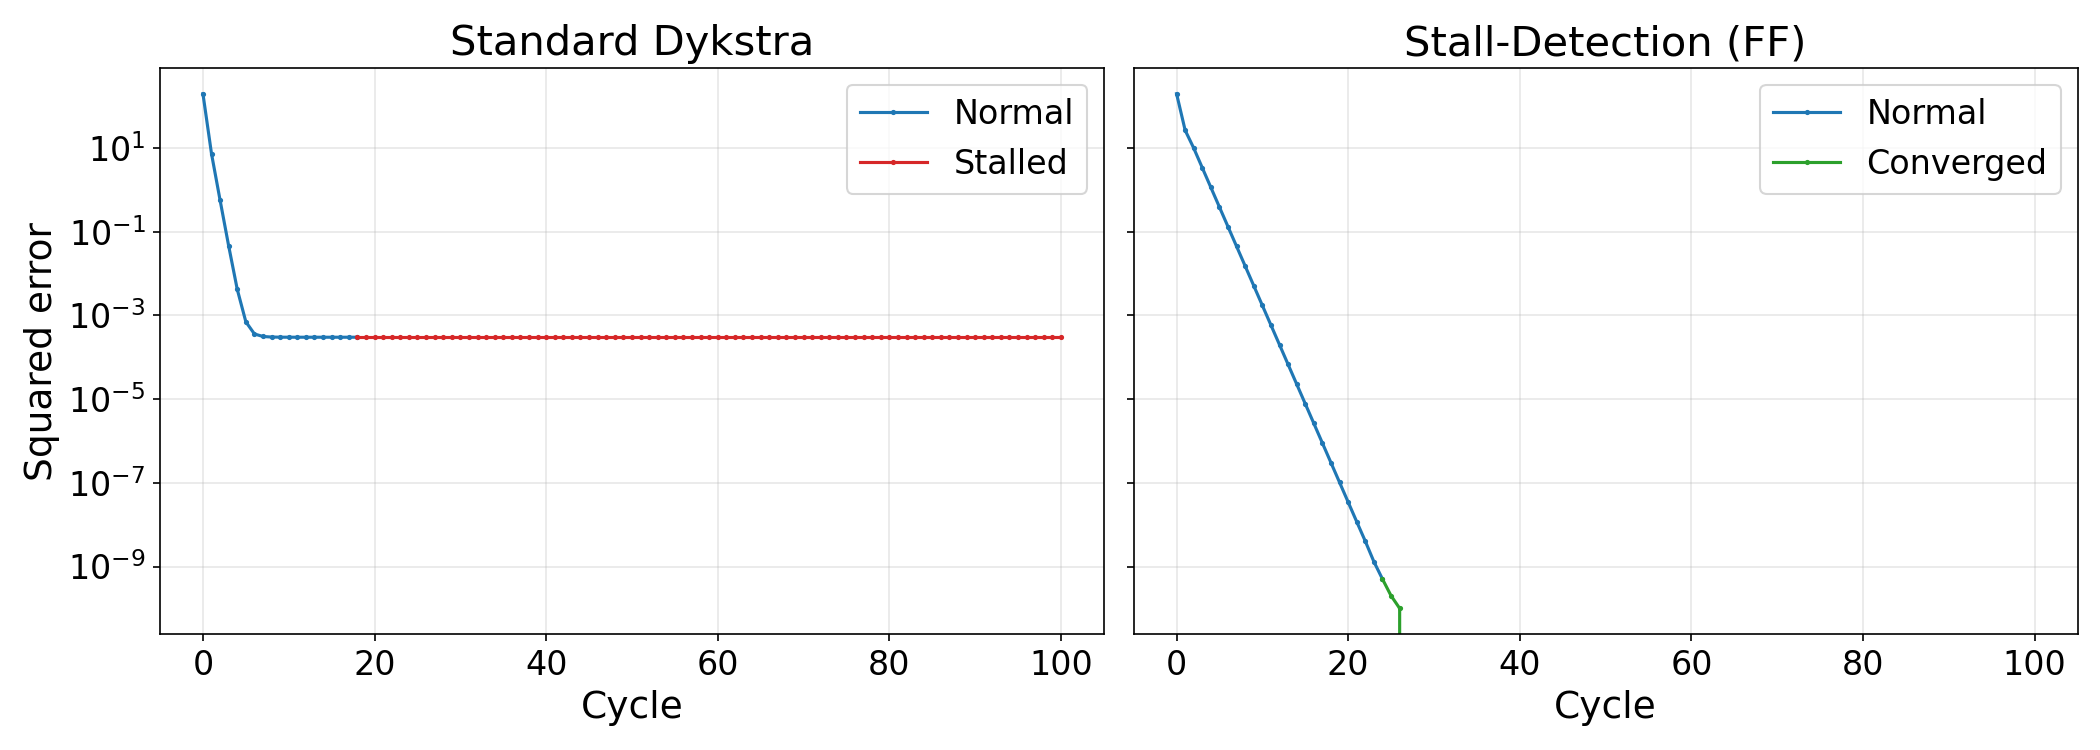
\includegraphics[width=\linewidth]{figures/benchmark_convergence_SEED=42_DIM=3_HS=6_EARLYTERMINATION.png}
        \caption{Convergence behaviour in three dimensions ($d=3$, $n=6$)}
        \label{fig:bench_3_6}
    \end{subfigure}
    
    \vspace{1em}
    
    \begin{subfigure}{\linewidth}
        \centering
        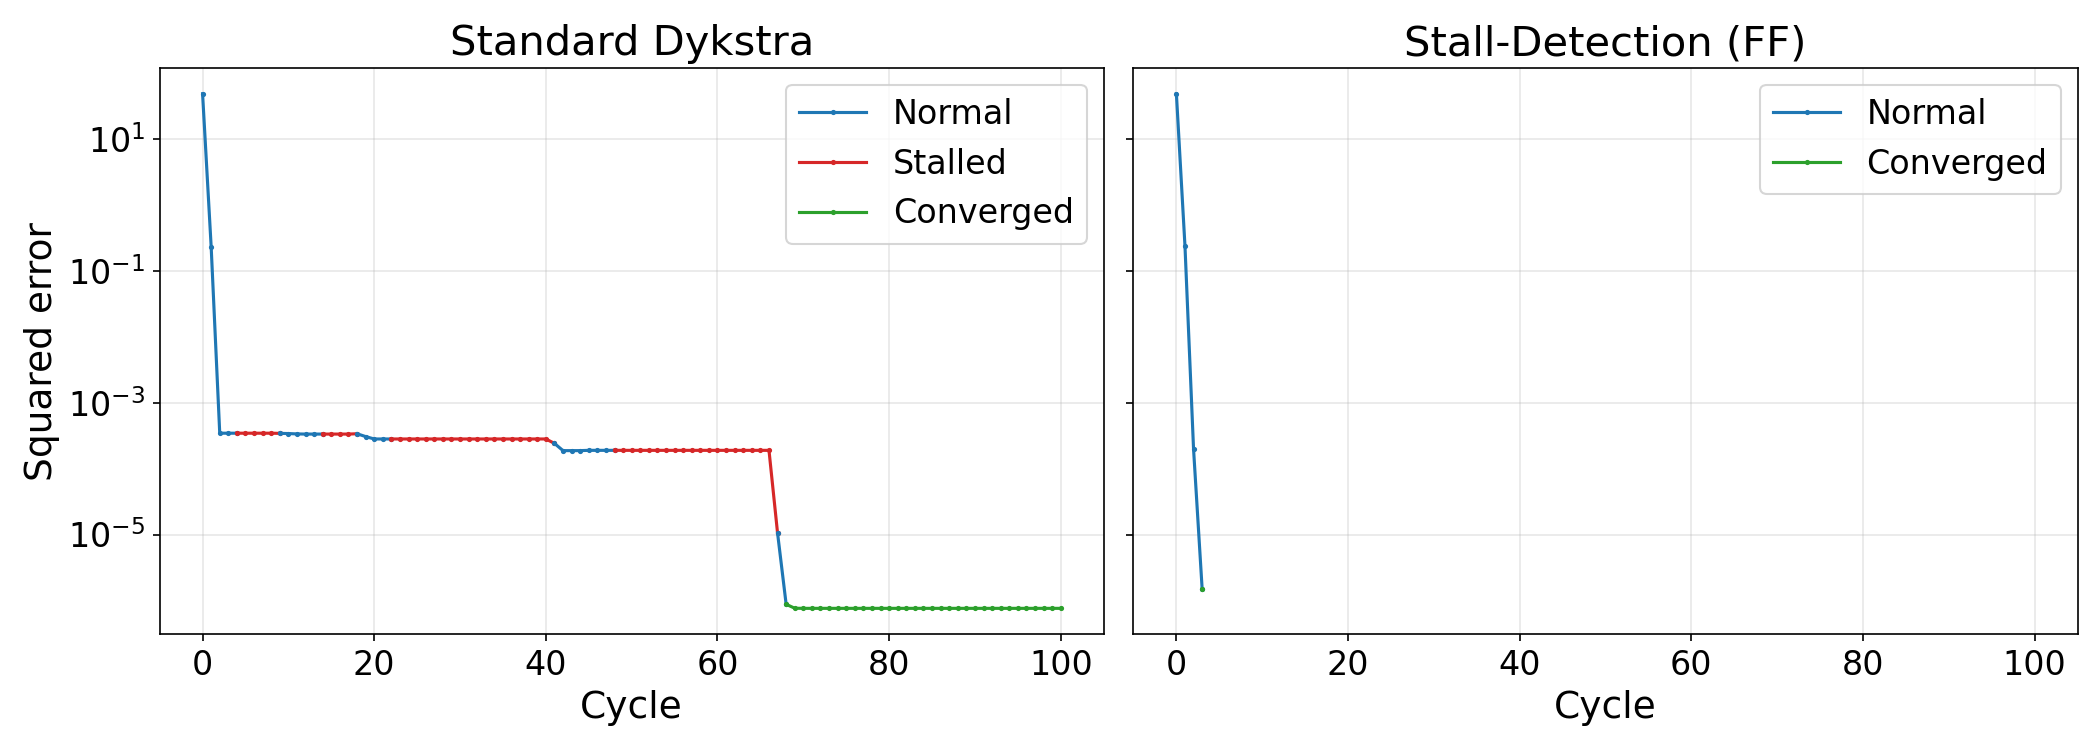
\includegraphics[width=\linewidth]{figures/benchmark_convergence_SEED=42_DIM=2_HS=20_EARLYTERMINATION.png}
        \caption{Convergence behaviour under a large number of polyhedral constraints ($d=2$, $n=20$)}
        \label{fig:bench_2_20}
    \end{subfigure}
    
    \vspace{1em}
    
    \begin{subfigure}{\linewidth}
        \centering
        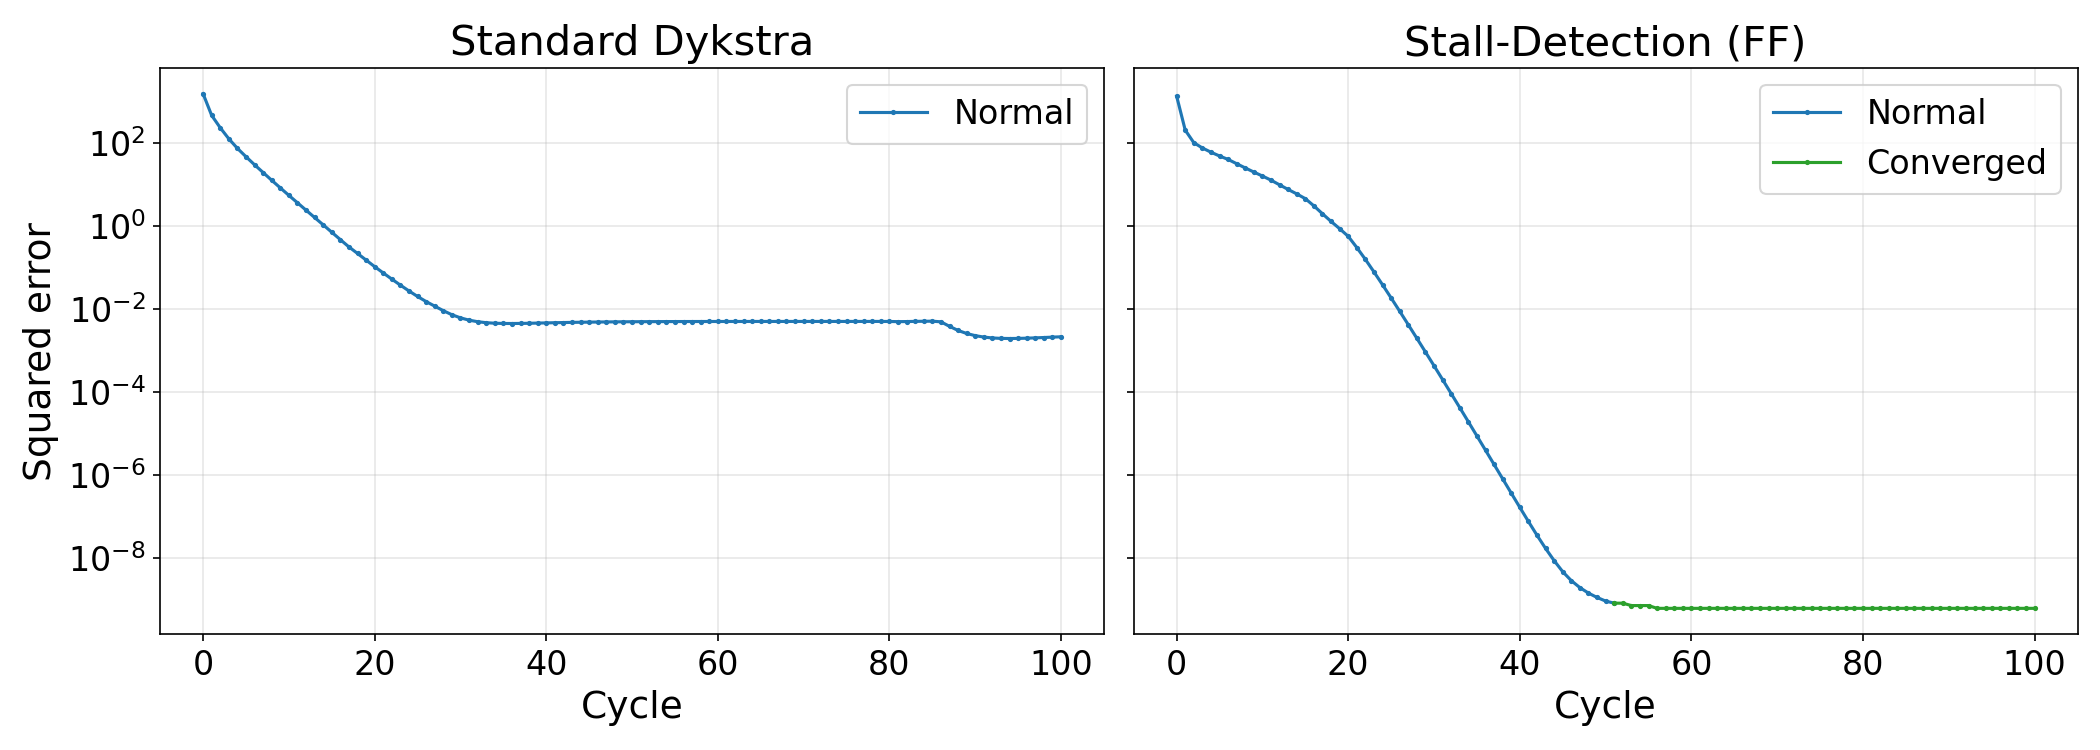
\includegraphics[width=\linewidth]{figures/benchmark_convergence_SEED=42_DIM=20_HS=50_EARLYTERMINATION.png}
        \caption{Convergence behaviour in high dimensions ($d=20$, $n=50$)}
        \label{fig:bench_20_50}
    \end{subfigure}
    
    \caption{Benchmark of Algorithm~\ref{alg:fastforward} versus Dykstra across varying geometries.}
    \label{fig:benchmark_convergence_stacked}
\end{figure}

Conversely, as seen across all three subfigures, Algorithm~\ref{alg:fastforward} eliminates the flat plateaus caused by stalling. In both low-dimensional cases (Figures~\ref{fig:bench_3_6}--\ref{fig:bench_2_20}), it breaks the initial gridlock and drives the spatial error down to high numerical precision in a handful of iterations Because the closed-form calculation proposed in Theorem~\ref{thm:nstall} relies exclusively on lightweight vector operations, the computational time overhead required to perform this detection and fast-forwarding is virtually negligible.

\begin{table}[htbp]
    \centering
    \caption{Runtime and final error across the benchmark environments.}
    \label{tab:benchmark_runtime}
    \begin{tabular}{@{}ccccc@{}}
        \toprule
        & \multicolumn{2}{c}{Standard Dykstra} & \multicolumn{2}{c}{Algorithm~\ref{alg:fastforward} (FF)} \\
        \cmidrule(lr){2-3} \cmidrule(l){4-5}
        Experiment & Time (s) & Final Error & Time (s) & Final Error \\
        \midrule
        (a) & 0.0275 & $3.01 \times 10^{-4}$ & 0.0134 & $0.00$ \\
        (b) & 0.0963 & $7.56 \times 10^{-7}$ & 0.0176 & $1.50 \times 10^{-7}$ \\
        (c) & 0.2811 & $2.15 \times 10^{-3}$ & 0.2261 & $6.00 \times 10^{-10}$ \\
        \bottomrule
    \end{tabular}
\end{table}

To quantify the direct computational advantages of bypassing stalling, the wall-clock execution time and the terminal squared spatial error $E(w^{(N_{\max})})$ were recorded for each scenario. As detailed in Table~\ref{tab:benchmark_runtime}, the fast-forward modification yields significant performance improvements across all tested geometries. In the low-dimensional configuration (a), the execution time is more than halved while driving the spatial error strictly to zero (finite-iteration convergence). Under the dense planar constraints of experiment (b), the solver achieves an 81\% reduction in runtime while maintaining comparable terminal precision. Most critically, in the high-dimensional regime (c), the modified algorithm not only reduces the overall computational runtime but also improves the final spatial accuracy by 7 orders of magnitude.
\section{Summary} \label{sec:dykstra_summary}

Dykstra's algorithm provides a computationally lightweight method for calculating Euclidean projections, yet the unpredictable stalling phenomenon has historically inhibited its deployment in time-critical and high-frequency engineering frameworks~\cite{DYKSTRASTALLING}. This chapter successfully resolved the stalling problem for polyhedral feasible regions. By formalising the cyclical mechanics of the primary and auxiliary variables during a stall (Section~\ref{sec:stalling_phenomenon}), we derived an exact, closed-form mathematical solution for its duration (Section~\ref{sec:closed_form_solution}). This derivation directly enabled the construction of a fast-forward modified solver (Section~\ref{sec:fast_forward_algorithm}) that actively monitors the stationarity condition and instantly advances the internal memory variables past the stalling cycles.

As demonstrated by the empirical benchmarks (Section~\ref{sec:dykstra_numerical_experiments}), this algorithmic modification eliminates computational gridlock across diverse pathological geometries. It systematically reduces wall-clock execution time and accelerates convergence while strictly preserving the asymptotic convergence guarantees of the baseline method (Corollary~\ref{cor:convergence}). The theoretical derivations and optimisation advancements detailed throughout this chapter have been formally published as a preprint as preprint in~\cite{Vestini2025}.

With this core mathematical foundation, the fast-forward projection solver is now transformed into a highly predictable, real-time computational engine for computing Euclidean projections. The thesis now pivots from pure optimisation to the applied aerospace domain. The subsequent chapters will leverage this fast-forward architecture to enforce structural constraints within the PGD learning framework, enabling the accurate tracking of highly non-linear satellite uncertainty in the cislunar environment via optimal transport.

\chapter{Optimal transport} \label{ch:optimal_transport}
Nonlinear physical dynamics, such as those governing cislunar aerospace applications, frequently distort initial uncertainties into complex, non-Gaussian probability distributions. Direct evaluation and filtering within these intractable target state spaces are computationally prohibitive. Optimal transport provides a theoretical mechanism to construct a deterministic coupling that pushes these complex target distributions forward to a simple, standard normal reference distribution, rendering subsequent analytical tasks mathematically tractable. However, guaranteeing that these transport maps remain physically valid and invertible requires strict adherence to monotonicity constraints, which inherently restricts the operational domain of the learning algorithm to a bounded feasible region.

In this chapter, we formulate a deterministic density estimation framework utilising the lower-triangular Knothe-Rosenblatt rearrangement. By parameterising the map components with a truncated probabilist's Hermite polynomial basis, we reformulate the infinite-dimensional map estimation task into a finite-dimensional, constrained maximum likelihood problem. The physical necessity of probability mass conservation dictates a dense system of linear inequality constraints evaluated over an empirical particle ensemble. This structural formulation forms the applied aerospace pillar of this thesis, directly establishing the exact polyhedral geometry and Constrained Quadratic Program (CQP) that necessitates the accelerated Dykstra projection algorithm developed in the preceding chapter.

\section*{Notation}
We denote the continuous state space as $\mathcal{X} \subseteq \mathbb{R}^d$, where $d$ is the spatial dimension. A discrete ensemble of particles drawn from the target measure is denoted by $x^{(i)}$, with the total empirical particle count fixed as $n$. The deterministic transport map is denoted as $S(x)$, and its individual scalar components are indicated by a superscript as $S^k(x)$. The partial derivative with respect to the $k$-th spatial coordinate is denoted by $\partial_k$. The probability density functions of the target and reference measures are denoted as $p(x)$ and $\eta(z)$, respectively. The univariate probabilist's Hermite polynomial of degree $m$ is denoted as $\mathrm{He}_m(\cdot)$, while the multivariate basis functions constructed via tensor products are denoted as $\Psi_j(x)$. The unknown scalar coefficients comprising the decision variable for the $k$-th map component are grouped in the vector $w^{(k)}$. The dense constraint matrix is denoted as $A$, and the resulting feasible polyhedral set enforcing physical monotonicity is denoted as $\mathcal{C}$.
\section{The Knothe-Rosenblatt rearrangement}
\label{sec:optimal_transport_kr}

The fundamental goal of optimal transport is to construct a deterministic coupling between two probability measures. We denote a continuous state space as $\mathcal{X} \subseteq \mathbb{R}^D$. We consider a target probability measure, which is often a complex and non-Gaussian distribution arising from nonlinear physical dynamics. In practice, this target distribution is analytically intractable to evaluate directly. Instead, we assume access to a discrete ensemble of $n$ samples, or particles, denoted by $\{x^{(1)}, \dots, x^{(n)}\} \subset \mathcal{X}$, drawn from this target distribution. 

Our overarching objective is to identify a deterministic transport map $S: \mathbb{R}^D \rightarrow \mathbb{R}^D$ that pushes the complex target distribution forward to a simple, well-characterised reference distribution. By transforming the particles into a domain where their distribution is known, subsequent analytical tasks in aerospace engineering, such as filtering or uncertainty propagation, become computationally tractable. We fix the reference measure as the standard multivariate normal distribution, $\mathcal{N}(0, I_D)$.

\begin{figure}[htbp]
    \centering
    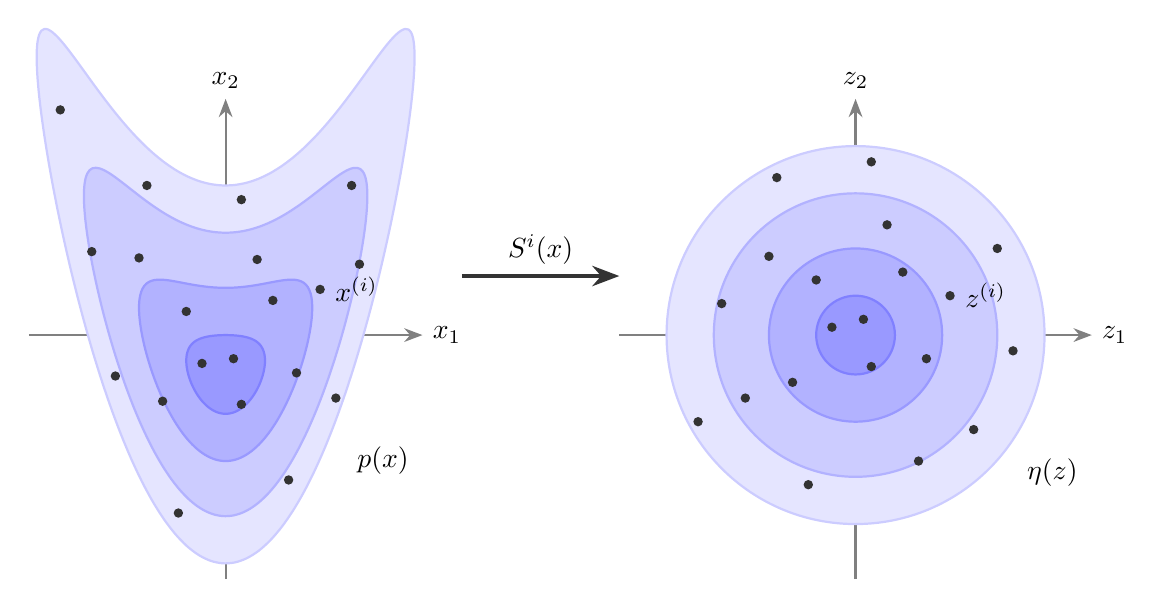
\begin{tikzpicture}[
        >=Stealth,
        particle/.style={circle, fill=black!80, inner sep=1.2pt},
        mapped_particle/.style={circle, fill=black!80, inner sep=1.2pt},
        axis/.style={->, gray, thick},
        contour1/.style={fill=blue!10, draw=blue!20, thick},
        contour2/.style={fill=blue!20, draw=blue!30, thick},
        contour3/.style={fill=blue!30, draw=blue!40, thick},
        contour4/.style={fill=blue!40, draw=blue!50, thick}
    ]
    
        \begin{scope}[shift={(0,0)}]

            \draw[axis] (-2.5, 0) -- (2.5, 0) node[right, text=black] {$x_1$};
            \draw[axis] (0, -3.1) -- (0, 3.0) node[above, text=black] {$x_2$};
            
            \draw[contour1] plot[domain=0:360, samples=100, smooth cycle] 
                ({2.4*cos(\x)}, {2.4*sin(\x) + 4.032*cos(\x)*cos(\x) - 0.5});
                
            \draw[contour2] plot[domain=0:360, samples=100, smooth cycle] 
                ({1.8*cos(\x)}, {1.8*sin(\x) + 2.268*cos(\x)*cos(\x) - 0.5});
                
            \draw[contour3] plot[domain=0:360, samples=100, smooth cycle] 
                ({1.1*cos(\x)}, {1.1*sin(\x) + 0.847*cos(\x)*cos(\x) - 0.5});
                
            \draw[contour4] plot[domain=0:360, samples=100, smooth cycle] 
                ({0.5*cos(\x)}, {0.5*sin(\x) + 0.175*cos(\x)*cos(\x) - 0.5});

            \node[particle] at (0.1, -0.3) {};
            \node[particle] at (-0.3, -0.36) {};
            \node[particle] at (0.2, -0.88) {};
            \node[particle] at (-0.5, 0.3) {};
            \node[particle] at (0.6, 0.44) {};
            \node[particle] at (0.9, -0.48) {};
            \node[particle] at (-0.8, -0.84) {};
            \node[particle] at (-1.1, 0.98) {};
            \node[particle] at (0.4, 0.96) {};
            \node[particle] at (-1.4, -0.52) {};
            \node[particle] at (1.4, -0.8) {};
            \node[particle] at (0.8, -1.84) {};
            \node[particle] at (-1.7, 1.06) {};
            \node[particle] at (1.6, 1.9) {};
            \node[particle] at (-0.6, -2.26) {};
            \node[particle] at (1.7, 0.9) {};
            \node[particle] at (-2.1, 2.86) {};
            \node[particle] at (0.2, 1.72) {};
            \node[particle] at (-1.0, 1.9) {};

            \node[particle] (xi) at (1.2, 0.58) {};
            \node[right=2pt] at (xi) {$x^{(i)}$};
            
            \node[below=0.3cm of {(2.0,-1.0)}] {$p(x)$};
        \end{scope}

        \draw[->, line width=1.5pt, color=black!80] (3.0, 0.75) -- (5.0, 0.75) node[midway, above, text=black] {$S^i(x)$};

        \begin{scope}[shift={(8.0, 0.0)}]
            \draw[axis] (-3.0, 0) -- (3.0, 0) node[right, text=black] {$z_1$};
            \draw[axis] (0, -3.1) -- (0, 3.0) node[above, text=black] {$z_2$};

            \draw[contour1] (0,0) circle (2.4);
            \draw[contour2] (0,0) circle (1.8);
            \draw[contour3] (0,0) circle (1.1);
            \draw[contour4] (0,0) circle (0.5);

            \node[mapped_particle] at (0.1, 0.2) {};
            \node[mapped_particle] at (-0.3, 0.1) {};
            \node[mapped_particle] at (0.2, -0.4) {};
            \node[mapped_particle] at (-0.5, 0.7) {};
            \node[mapped_particle] at (0.6, 0.8) {};
            \node[mapped_particle] at (0.9, -0.3) {};
            \node[mapped_particle] at (-0.8, -0.6) {};
            \node[mapped_particle] at (-1.1, 1.0) {};
            \node[mapped_particle] at (0.4, 1.4) {};
            \node[mapped_particle] at (-1.4, -0.8) {};
            \node[mapped_particle] at (1.5, -1.2) {};
            \node[mapped_particle] at (0.8, -1.6) {};
            \node[mapped_particle] at (-1.7, 0.4) {};
            \node[mapped_particle] at (1.8, 1.1) {};
            \node[mapped_particle] at (-0.6, -1.9) {};
            \node[mapped_particle] at (2.0, -0.2) {};
            \node[mapped_particle] at (-2.0, -1.1) {};
            \node[mapped_particle] at (0.2, 2.2) {};
            \node[mapped_particle] at (-1.0, 2.0) {};
            
            \node[mapped_particle] (zi) at (1.2, 0.5) {};
            \node[right=2pt] at (zi) {$z^{(i)}$};

            \node[below=0.45cm of {(2.5,-1.0)}] { $\eta(z)$};
        \end{scope}

    \end{tikzpicture}
    \caption{A schematic illustrating optimal transport via a deterministic map $S$.}
    \label{fig:optimal_transport_schematic}
\end{figure}

The problem of finding a valid transport map $S$ such that the pushforward of the target measure equals the reference measure is highly underdetermined; without further constraints, there exist infinitely many such couplings. To render the problem identifiable, we restrict our hypothesis space to the Knothe-Rosenblatt (KR) rearrangement. The KR map is strictly defined by two structural properties: it is lower-triangular, and it is strictly monotone~\cite{Baptista2022}. We partition the map into its scalar components as
\begin{equation*}
    S(x) = \begin{bmatrix} S^1(x_1) \\ S^2(x_1, x_2) \\ \vdots \\ S^D(x_1, \dots, x_d) \end{bmatrix}.
    \label{eq:kr_map_structure}
\end{equation*}

To push one continuous measure forward to another while maintaining a valid probability density, the transport map must be a \emph{global diffeomorphism}, a continuously differentiable, bijective mapping. Bijectivity guarantees that the transformation is invertible and that disparate physical states in the target space do not map to the identical coordinate in the reference space. Thus, to ensure the map $S$ conserves probability mass and is invertible, the map must be \emph{monotonic}~\cite{Baptista2022}. 

The lower-triangular structure ensures that the Jacobian matrix of the map, $\nabla S(x)$, is inherently lower-triangular. Recall that the determinant of a triangular matrix is given by the product of its diagonal entries. The monotonicity constraint thus dictates that each individual component $S^k$ must be a strictly increasing function with respect to its own $k$-th argument. Using $\partial_k$ to denote the partial derivative with respect to the $k$-th variable, we require
\begin{equation}
    \boxed{
    \partial_k S^k(x) > 0 \quad \forall k \in \{1, \dots, d\}}.
    \label{eq:monotonicity_continuous}
\end{equation}

To find the optimal map, we frame the task as a density estimation problem. We denote the unknown probability density function of the target distribution as $p(\cdot)$ and the probability density function of the standard normal reference distribution as $\eta(\cdot)$. By the fundamental change of variables formula for probability density functions, the target density evaluated at a spatial coordinate $x$ is given by
\begin{equation*}
    p(x) = \eta(S(x)) \det \nabla S(x).
    \label{eq:change_of_variables}
\end{equation*}

To construct a maximum likelihood estimator, we evaluate the logarithm of the target density. Taking the natural logarithm of both sides yields
\begin{equation*}
    \log p(x) = \log \eta(S(x)) + \log \det \nabla S(x).
    \label{eq:log_density_initial}
\end{equation*}

Because the chosen reference distribution is a standard multivariate normal, its $d$ spatial components are mutually independent. The density function is $\eta(z) \propto \exp\left(-\frac{1}{2} \|z\|_{2}^2\right)$, meaning the log-density is proportional to $-\frac{1}{2}\|S(x)\|_{2}^2$. Furthermore, substituting the product of the diagonal elements for the determinant of the Jacobian simplifies the log-determinant term into a summation. Applying these substitutions yields
\begin{equation*}
    \log p(x) \propto -\frac{1}{2} \|S(x)\|_{2}^2 + \log \left( \prod_{k=1}^d \partial_k S^k(x) \right) = -\frac{1}{2} \|S(x)\|_{2}^2 + \sum_{k=1}^d \log \partial_k S^k(x).
    \label{eq:log_density_expanded}
\end{equation*}

Following a \emph{maximum likelihood estimation} approach, we seek to find the map $S$ that maximises the expected log-likelihood of the observed data, which is mathematically equivalent to minimising the negative log-likelihood evaluated over the $n$ empirical particles~\cite{Baptista2022}. Averaging across all particles $x^{(i)}$, and flipping signs, gives the empirical objective function:
\begin{equation*}
    \min_{S} \frac{1}{n} \sum_{i=1}^n \left( \frac{1}{2} \|S(x^{(i)})\|_{2}^2 - \sum_{k=1}^d \log \partial_k S^k(x^{(i)}) \right).
    \label{eq:full_negative_log_likelihood}
\end{equation*}

We write the squared $\ell_2$-norm explicitly as the sum of its squared components, $\|S(x)\|_{2}^2 = \sum_{k=1}^D (S^k(x))^2$. Substituting and rearranging the order of summation yields:
\begin{equation*}
    \min_{S} \sum_{k=1}^D \left[ \frac{1}{n} \sum_{i=1}^n \left( \frac{1}{2} (S^k(x^{(i)}))^2 - \log \partial_k S^k(x^{(i)}) \right) \right].
    \label{eq:decoupled_likelihood}
\end{equation*}

It is now evident that the objective function completely decouples. The terms associated with any specific map component $S^k$ do not depend on any other component $S^j$ for $j \neq k$. This property allows us to separate the computationally demanding high-dimensional optimisation problem into $D$ independent scalar estimation problems. For any given $k$-th dimension of the state space, the optimal map component is obtained by solving
\begin{equation}
    \boxed{
    \min_{S^k \in \mathcal{S}_k} \frac{1}{n} \sum_{i=1}^n \left( \frac{1}{2} (S^k(x^{(i)}))^2 - \log \partial_k S^k(x^{(i)}) \right)
    }.
    \label{eq:mle_objective}
\end{equation}
Here, $\mathcal{S}_k$ represents the infinite-dimensional hypothesis space of all functions that satisfy the monotonicity constraint defined in \eqref{eq:monotonicity_continuous}. 

The objective function in \eqref{eq:mle_objective} balances two simultaneous demands. The quadratic term encourages the mapped particles to cluster near the origin, adopting the unit variance of the standard normal reference. Simultaneously, the logarithmic term severely penalises maps that compress the probability space towards zero, thereby preventing the formation of singular transformations. The formulation up to this point is continuous and infinite-dimensional; practically, to apply numerical optimisation techniques to learn the map, we must parameterise $\mathcal{S}_k$ using a finite-dimensional polynomial basis.
\section{Hermite polynomial parameterisation} \label{sec:hermite_basis}

To solve the independent scalar estimation problems computationally, we must project the infinite-dimensional hypothesis space $\mathcal{S}_k$ into a finite-dimensional functional basis. The choice of basis is critical for the numerical stability of the optimisation routine. Utilising a standard monomial basis to expand the transport map yields severely ill-conditioned linear systems when evaluating expectations against a Gaussian measure, impairing the convergence of gradient-based solvers. Because our objective function inherently assumes the mapped particles follow a standard normal reference distribution, we construct the basis using probabilist's Hermite polynomials. These polynomials are orthogonal with respect to the standard normal probability density function, which smooths the optimisation landscape.

We define the sequence of univariate probabilist's Hermite polynomials, $\mathrm{He}_m(y)$ for a scalar input $y$ and degree $m$, via the recurrence relation:
\begin{align}
    \mathrm{He}_0(y) &= 1, \nonumber \\
    \mathrm{He}_1(y) &= y, \nonumber \\
    \mathrm{He}_{m+1}(y) &= y \mathrm{He}_m(y) - m \mathrm{He}_{m-1}(y).
    \label{eq:hermite_recurrence}
\end{align}

\begin{figure}[htbp]
    \centering
    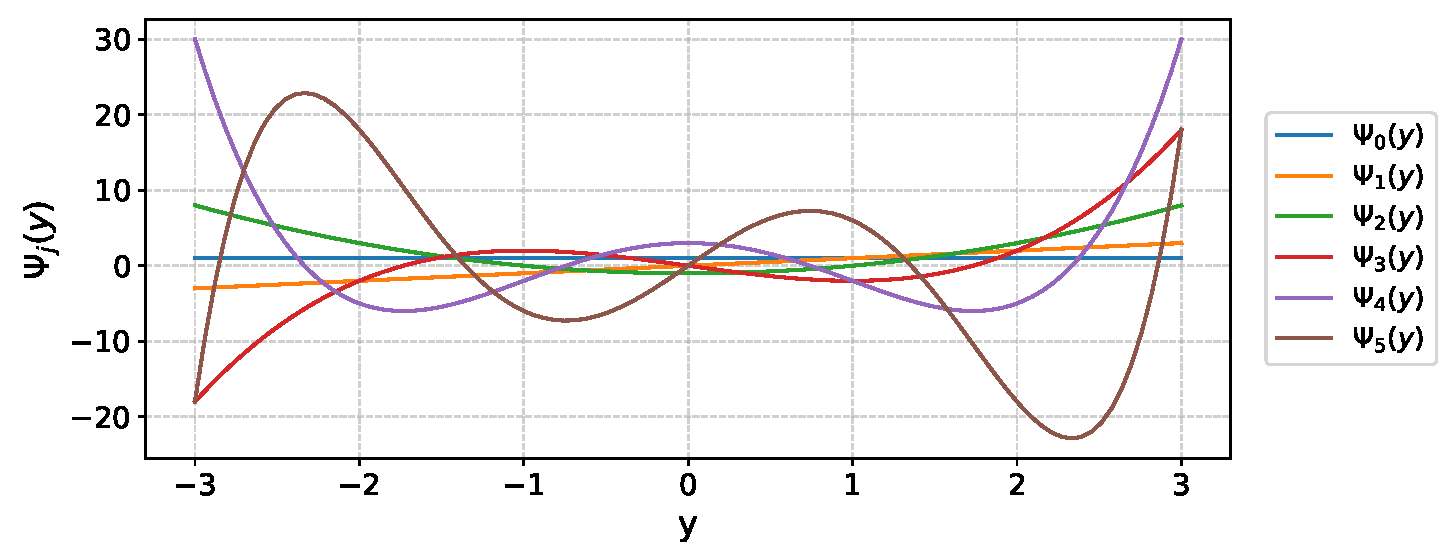
\includegraphics[width=\linewidth]{figures/Hermite.pdf}
    \caption{The first five Hermite polynomials evaluated over the real line.}
    \label{fig:hermite_polynomials}
\end{figure}

As illustrated in Figure~\ref{fig:hermite_polynomials}, the polynomials exhibit structural zero-crossings and growth rates that are well-suited for capturing the variations of a probability density. To parameterise the full multivariate transport map, we require multivariate basis functions. For the $k$-th component of the map, the function depends strictly on the first $k$ spatial coordinates, $x_1, \dots, x_k$, to enforce the lower-triangular structure of the Knothe-Rosenblatt rearrangement. We construct multivariate basis functions, $\Psi_j(x)$, by taking the tensor product of the univariate Hermite polynomials across these $k$ active dimensions. 

A full tensor product basis up to a maximum polynomial degree $D$ contains $(D+1)^k$ terms. For high-dimensional state spaces encountered in aerospace tracking problems, this exponential growth in decision variables renders the parameterisation computationally intractable. To alleviate this dimensionality issue, we enforce a priori mathematical sparsity through total degree truncation. We construct a filtered index set where a tensor product term is only retained if the sum of its univariate polynomial degrees is less than or equal to $D$. This truncation strategy limits the size of the basis while preserving the expressivity required to invert the physical nonlinear shears of the target distribution.

We denote the number of retained basis functions for the $k$-th map component as $J_k + 1$. We approximate the scalar map component using a linear combination of these basis functions:
\begin{equation}
    S^k(x) = \sum_{j=0}^{J_k} w_j^{(k)} \Psi_j(x),
    \label{eq:hermite_expansion}
\end{equation}
where the vector $w^{(k)} \in \mathbb{R}^{J_k+1}$ contains the unknown scalar coefficients that we must optimise. 

A direct mathematical advantage of this specific parameterisation emerges when evaluating the strict monotonicity constraint, $\partial_k S^k(x) > 0$. The derivative of a probabilist's Hermite polynomial obeys the linear relation:
\begin{equation}
    \frac{d}{dy} \mathrm{He}_m(y) = m \mathrm{He}_{m-1}(y).
    \label{eq:hermite_derivative}
\end{equation}
Because $\Psi_j(x)$ is a tensor product, the partial derivative $\partial_k$ only operates on the univariate polynomial associated with the $k$-th spatial coordinate, $x_k$. Consequently, the partial derivative of the map component reduces to a linear combination of lower-degree Hermite polynomials, evaluated strictly with respect to the decision variables $w^{(k)}$:
\begin{equation}
    \partial_k S^k(x) = \sum_{j=0}^{J_k} w_j^{(k)} \partial_k \Psi_j(x).
    \label{eq:map_derivative_linear}
\end{equation}
Substituting the finite expansion \eqref{eq:hermite_expansion} and its linear derivative \eqref{eq:map_derivative_linear} into the infinite-dimensional continuous objective \eqref{eq:mle_objective} reformulates the density estimation task as a finite-dimensional optimisation problem.
\section{Constrained optimisation formulation} \label{sec:constrained_optimisation}

Having parameterised the scalar map component using a truncated Hermite polynomial basis, we can substitute the finite expansion \eqref{eq:hermite_expansion} and its linear derivative \eqref{eq:map_derivative_linear} directly into the continuous negative log-likelihood \eqref{eq:mle_objective}. For a specific $k$-th dimension of the state space, the density estimation task becomes a finite-dimensional optimisation problem over the unknown coefficient vector $w^{(k)} \in \mathbb{R}^{J_k+1}$. We define the resulting empirical objective function as
\begin{equation}
    f(w^{(k)}) = \frac{1}{n} \sum_{i=1}^n \left( \frac{1}{2} \left( \sum_{j=0}^{J_k} w_j^{(k)} \Psi_j(x^{(i)}) \right)^2 - \log \left( \sum_{j=0}^{J_k} w_j^{(k)} \partial_k \Psi_j(x^{(i)}) \right) \right).
    \label{eq:finite_objective}
\end{equation}
Because the quadratic penalty is strictly convex and the negative logarithm is strictly convex over its positive domain, the composite objective function $f(w^{(k)})$ is strictly convex with respect to the decision variables $w^{(k)}$.

To ensure the map remains a global diffeomorphism, we must formally impose the strict monotonicity constraint $\partial_k S^k(x) > 0$. Because we only possess empirical access to the target distribution via the $n$ discrete samples, we enforce this constraint exactly at every observed particle. Furthermore, to ensure numerical stability and rigorously avoid boundary cases that could momentarily fold the probability mass during the iterative learning process, we introduce a strictly positive tolerance parameter $\varepsilon > 0$. The monotonicity condition evaluated at an arbitrary particle $x^{(i)}$ therefore becomes
\begin{equation}
    \sum_{j=0}^{J_k} w_j^{(k)} \partial_k \Psi_j(x^{(i)}) \ge \varepsilon.
    \label{eq:discrete_monotonicity}
\end{equation}

By exploiting the linearity of the derivative operator across the polynomial basis, the condition in \eqref{eq:discrete_monotonicity} constitutes a purely linear inequality constraint on the decision variables. By evaluating these basis derivatives at every particle $x^{(i)}$ in the ensemble and stacking the results, we construct a dense constraint matrix $A \in \mathbb{R}^{n \times (J_k+1)}$. Each row of $A$ represents the gradient information evaluated at a single spatial location. We define a vector $\epsilon \in \mathbb{R}^n$ where every entry is equal to the small positive scalar $\varepsilon$. This transforms the $n$ distinct physical constraints into a unified matrix inequality:
\begin{equation}
    A w^{(k)} \ge \epsilon \quad \implies \quad -A w^{(k)} \le -\epsilon.
    \label{eq:matrix_inequality}
\end{equation}

This system of linear inequalities strictly bounds the operational domain of our solver. Geometrically, each row of the matrix $-A$ defines a distinct closed half-space in the high-dimensional coefficient space. The feasible region for the optimal map coefficients is defined by the intersection of these $n$ half-spaces, forming a dense polyhedral set, which we denote as $\mathcal{C}$:
\begin{equation}
    \mathcal{C} = \left\{ w \in \mathbb{R}^{J_k+1} \mid -A w \le -\epsilon \right\}.
    \label{eq:polyhedral_set}
\end{equation}

Our overarching mathematical objective is to find the coefficient vector $w^{(k)}$ that minimises the unconstrained, strictly convex objective $f(w^{(k)})$ subject to the restriction that $w^{(k)} \in \mathcal{C}$. To navigate this constrained landscape, we implement a Projected Gradient Descent framework. In this approach, we compute the gradient of the objective and take an unconstrained descent step, resulting in an intermediate, unconstrained point which we shall denote $w^\circ$. 

Because the unconstrained point $w^\circ$ will frequently violate the monotonicity conditions (i.e., $w^\circ \notin \mathcal{C}$), we must rigorously enforce the physical reality of the problem by projecting the point back onto the feasible polyhedral intersection. This projection must alter the learned coefficients as minimally as possible to retain the maximum likelihood data. Therefore, the projection operation requires us to find the unique point $w^\star \in \mathcal{C}$ that minimises the Euclidean distance to the unconstrained point $w^\circ$. Mathematically, this is equivalent to solving the following Constrained Quadratic Program (CQP):
\begin{equation}
\begin{array}{ll}
    \displaystyle \minimise_{w \in \mathbb{R}^{J_k+1}} & \frac{1}{2}\|w - w^\circ\|_{\ell_2}^2 \\
    \text{subject to} & -Aw \le -\epsilon.
\end{array}
\label{eq:cqp_projection}
\end{equation}

Solving this specific exact Euclidean projection problem forms the fundamental bridge between the optimal transport framework defined in this chapter and the accelerated projection algorithms derived previously. The robust numerical solution of \eqref{eq:cqp_projection} across tens of thousands of learning iterations is the computational engine of this thesis.
\section{Summary} \label{sec:optimal_transport_summary}

This chapter outlined the mathematical foundation of the optimal transport framework adopted in this thesis. Our overarching objective is to find the coefficient vector that minimises the objective $f(w^{(k)})$ defined in~\eqref{eq:finite_objective} subject to constraint $w^{(k)} \in \mathcal{H}$.

\subsection{Connection with Dykstra's algorithm}

To navigate this constrained landscape, we implement a Projected Gradient Descent (PGD) framework. In this approach (which we will treat in more detail in Chapter~\ref{ch:optimisation}), we compute the gradient of the objective and take an unconstrained descent step, resulting in an intermediate, unconstrained point which we denote $w^\circ$. 

Since the unconstrained point $w^\circ$ will frequently violate the monotonicity conditions (i.e., $w^\circ \notin \mathcal{H}$), we must project it back onto the feasible polyhedral intersection at each PGD iteration. This projection must alter the learned coefficients as minimally as possible to retain the maximum likelihood data. Therefore, the projection operation requires us to find the unique point $w^\star \in \mathcal{H}$ that minimises the Euclidean distance to the unconstrained point $w^\circ$. Mathematically, this is equivalent to solving the following CQP:
\begin{equation}
\begin{array}{ll}
    \displaystyle \minimise_{w \in \mathbb{R}^{d}} & \frac{1}{2}\|w - w^\circ\|_{2}^2 \\
    \text{subject to} & -Aw \le -\epsilon_m.
\end{array}
\label{eq:cqp_projection}
\end{equation}

This formulation is equivalent to~\ref{eq:projection}. Solving this Euclidean projection problem at each PGD iteration bridges the optimal transport framework defined in this chapter and the fast-forward Dykstra algorithm (Algorithm~\ref{alg:fastforward}) derived in Chapter~\ref{ch:dykstra}.

\chapter{A highly scalable inexact projection framework} \label{ch:optimisation}
Finding optimal transport map components requires navigating a high-dimensional polynomial coefficient space to minimise the empirical log-likelihood subject to polyhedral monotonicity constraints. To solve this constrained problem efficiently across large particle sets, we introduce a highly scalable, inexact Projected Gradient Descent (PGD) architecture. The framework integrates stochastic gradient evaluation to navigate complex objective landscapes, iterative hard thresholding to enforce structural sparsity, and dynamic projection scheduling to circumvent the prohibitive computational costs of exact Euclidean projections.

\section*{Notation}
We denote set cardinality as $|\cdot|$. The Hadamard product, denoted by the operator $\odot$, represents the element-wise multiplication of two vectors or matrices of identical dimensions.
The outer learning PGD loop is indexed by $t \in \{0, 1, \dots, T-1\}$, where $T-1$ is the outer loop iteration budget, while the inner Dykstra projection cycle is indexed by $m$ and constrained by a dynamic iteration ceiling $M^{(t)}$, which scales according to a base budget $M_{\mathrm{base}}$ and an inexact growth exponent $p$. The stochastic gradient $g^{(t)}$ is evaluated over a random subset of particle indices $\mathcal{B}^{(t)} \subset \{1, 2, \dots, n\}$ with cardinality $B$. The learning rate is denoted as $\eta^{(t)}$, and decays according to an initial rate $\eta^\circ$ and a decay parameter $\gamma$. For the iterative hard thresholding procedure, we define a boolean active mask vector $\mathcal{M}^{(t)}$.


\section{Outer loop projected gradient descent}
\label{sec:outer_loop_pgd}

The density estimation framework formulated in Section~\ref{sec:constrained_optimisation} requires the minimisation of the convex empirical objective $f(\cdot)$ defined in \eqref{eq:finite_objective}, subject to the polyhedral feasible set $\mathcal{H}$ defined in \eqref{eq:polyhedral_set}. To navigate this constrained polynomial coefficient space and compute the optimal transport map, we deploy a PGD architecture. The PGD algorithm operates an outer learning loop, indexed by $t$, which iteratively updates the decision variables governing the map. Each outer iteration comprises two sequential mathematical operations: an unconstrained descent step evaluated over the target distribution, followed by an exact Euclidean projection to enforce physical monotonicity. 

In the first operation, we compute the gradient of the objective function evaluated at the current feasible iterate, $\nabla f(w^{(t)})$. The algorithm takes an unconstrained step in the direction of the negative gradient, scaled by a \emph{step size} (or \emph{learning rate}) parameter $\eta^{(t)}$. This operation produces an intermediate, potentially infeasible coefficient vector $w^{\circ}$:
\begin{equation}
    w^{\circ} = w^{(t)} - \eta^{(t)} \nabla f(w^{(t)}).
    \label{eq:pgd_unconstrained_gradient_step}
\end{equation}

The learning rate schedule follows an inverse time decay model $\eta^{(t)} = \eta^\circ / (1 + \gamma t)$, where $\eta^\circ \in \mathbb{R}$ is the initial learning rate and $\gamma \in \mathbb{R}$ is a decay coefficient. This decay mechanism helps the optimiser settle into narrow minima as the gradients decrease in magnitude during later iterations. This inverse model is visualised in Figure~\ref{fig:learning_rate_decay}, evaluated with an initial learning rate of $\eta^\circ = 0.1$ across varying decay coefficients $\gamma$.

\begin{figure}[htpb]
    \centering
    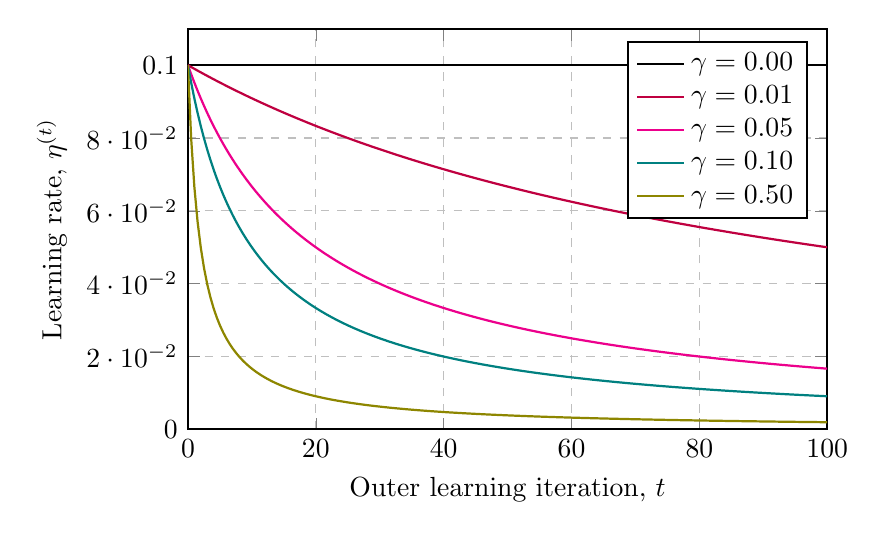
\begin{tikzpicture}
        \begin{axis}[
            width=0.8\textwidth,
            height=0.55\textwidth,
            xlabel={Outer learning iteration, $t$},
            ylabel={Learning rate, $\eta^{(t)}$},
            xmin=0, xmax=100,
            ymin=0, ymax=0.11,
            grid=major,
            grid style={dashed, gray!50},
            legend pos=north east,
            legend cell align={left},
            thick
        ]
        
        \addplot[domain=0:100, samples=200, color=black] {0.1 / (1 + 0*x)};
        \addlegendentry{$\gamma = 0.00$}
        
        \addplot[domain=0:100, samples=200, color=purple] {0.1 / (1 + 0.01*x)};
        \addlegendentry{$\gamma = 0.01$}
        
        \addplot[domain=0:100, samples=200, color=magenta] {0.1 / (1 + 0.05*x)};
        \addlegendentry{$\gamma = 0.05$}
        
        \addplot[domain=0:100, samples=200, color=teal] {0.1 / (1 + 0.1*x)};
        \addlegendentry{$\gamma = 0.10$}
        
        \addplot[domain=0:100, samples=200, color=olive] {0.1 / (1 + 0.5*x)};
        \addlegendentry{$\gamma = 0.50$}
        
        \end{axis}
    \end{tikzpicture}
    \caption{Inverse time decay schedule for the unconstrained learning rate.}
    \label{fig:learning_rate_decay}
\end{figure}
The selection of the decay coefficient $\gamma$ strictly governs the exploration-exploitation trade-off during the unconstrained descent phase. A value of $\gamma = 0$ reduces the schedule to a constant learning rate. While a constant step size promotes continuous exploration of the objective landscape, it frequently induces numerical oscillations around the optimal parameters and prevents the algorithm from converging to a precise local minimum. Conversely, an aggressive decay rate (e.g., $\gamma \ge 0.1$) rapidly diminishes the step size. This forces the optimiser to exploit the local geometry and settle quickly, but risks premature convergence to shallow, sub-optimal minima if deployed before the iterates reach the primary basin of attraction. A moderate decay provides a structural balance, allowing the framework to traverse flat ravines during the early learning iterations while ensuring the step size becomes sufficiently small to satisfy strict polyhedral feasibility constraints as $t$ approaches $T-1$.

Because this unconstrained step is driven solely by the maximum likelihood objective, it does not guarantee adherence to the structural constraints. The intermediate vector $w^{\circ}$ will frequently exit the feasible polyhedral intersection $\mathcal{H}$, corresponding to a transport map that temporarily violates the monotonicity requirement.

To rectify this and ensure the map remains strictly monotonic at every learning iteration, the second operation requires projecting $w^{\circ}$ back onto $\mathcal{H}$. This requires finding the unique feasible point that minimises the Euclidean distance to $w^{\circ}$, which is mathematically equivalent to solving the CQP defined in \eqref{eq:cqp_projection}. We denote the exact Euclidean projection operator onto the set $\mathcal{H}$ as $\mathcal{P}_{\mathcal{H}}(\cdot)$. The projected point becomes the feasible update for the subsequent learning iteration:
\begin{equation}
    w^{(t+1)} = \mathcal{P}_{\mathcal{H}}(w^\circ).
    \label{eq:pgd_projection_step}
\end{equation}

Within this framework, the evaluation of the projection operator $\mathcal{P}_{\mathcal{H}}(\cdot)$ acts as a direct function call to the accelerated Dykstra algorithm developed in Chapter~\ref{ch:dykstra}. The integration of the inner projection solver with this outer learning loop, including the dynamic parameterisation of the projection iteration limits and other computational optimisation techniques adopted, is detailed further in Section~\ref{sec:inner_loop_integration}.

The backbone of our PGD implementation therefore consists of applying the unconstrained gradient descent update~\eqref{eq:pgd_unconstrained_gradient_step} followed by the projection step~\eqref{eq:pgd_projection_step}. However, evaluating the deterministic gradient over the complete particle set at every iteration is computationally expensive and leaves the optimiser susceptible to ``slowing down'' in flat ravines within the objective landscape. To address these limitations and scale the framework, we replace the full-batch gradient evaluation with a stochastic approximation.
\section{Stochastic gradient descent and minibatching} \label{sec:sgd_minibatching}

In a traditional gradient descent framework, evaluating the exact gradient requires computing $\nabla f_i(w)$ for every index within the full particle set $\mathcal{I} = \{1, 2, \dots, n\}$. When $n$ is large, this full-batch computation introduces a severe computational bottleneck. To mitigate these computational and geometric challenges, we replace the full-batch gradient with a stochastic approximation. This technique is fundamentally rooted in the stochastic approximation methods developed by Robbins and Monro~\cite{Robbins1951} and has been extensively adapted for large-scale machine learning applications~\cite{Bottou2010}. By evaluating the gradient on a random subset of the data, Stochastic Gradient Descent (SGD) introduces inherent variance into the parameter updates. This stochastic noise disrupts deterministic ``slowing-down'', providing the iterates with the requisite momentum to escape near-flat ravines.

Mathematically, we define a mini-batch subset $\mathcal{B}^{(t)} \subset \mathcal{I}$, which is sampled uniformly at random without replacement at each outer learning iteration $t$. The cardinality of this subset is the mini-batch size $B = |\mathcal{B}^{(t)}|$, chosen such that $B \ll n$. By decomposing the primary objective function into individual particle contributions, $f_i(w)$, we compute the stochastic gradient $g^{(t)}$ as the sample mean over the mini-batch:
\begin{equation*}
    g^{(t)} = \frac{1}{B} \sum_{i \in \mathcal{B}^{(t)}} \nabla f_i(w^{(t)}).
    \label{eq:stochastic_gradient}
\end{equation*}
The vector $g^{(t)}$ serves as an unbiased estimator of the true full-batch gradient and replaces the deterministic term $\nabla f(w^{(t)})$ during the unconstrained descent phase.

While stochastic evaluation accelerates the unconstrained descent phase, we isolate this mini-batching logic from the inner projection loop. If we were to apply mini-batching to the projection operation, Dykstra's algorithm would only evaluate the subset of half-space constraints corresponding to the sampled particles in $\mathcal{B}^{(t)}$. Consequently, the intermediate projection would enforce $-A_{\mathcal{B}^{(t)}} w \le -\epsilon_{m, \mathcal{B}^{(t)}}$ rather than the complete polyhedral intersection $\mathcal{H}$. The unconstrained step explores the parameter space stochastically using $B$ samples, while the Euclidean projection $\mathcal{P}_{\mathcal{H}}(\cdot)$ enforces the global geometry of all $n$ half-spaces. This dual approach ensures computational scalability while guaranteeing the transport map remains a valid physical diffeomorphism at every iteration.
\section{Iterative hard thresholding} \label{sec:iht}

As the spatial dimension of the physical system increases, the number of polynomial coefficients parameterising the Knothe-Rosenblatt map scales rapidly. Although the total degree truncation introduced in Chapter~\ref{ch:optimal_transport} provides \emph{a priori} structural sparsity, the continuous optimisation process will nonetheless assign non-zero yet values to basis terms that possess no physical significance. Over thousands of learning iterations, these numerical artifacts accumulate, degrading computational efficiency and generalisation.

To enforce physical sparsity during the training process, we incorporate Iterative Hard Thresholding (IHT) into the outer learning loop. IHT functions as a periodic filtering mechanism that evaluates the magnitude of the coefficient iterates and forcibly zeroes out any terms falling below a designated scalar tolerance. Once a coefficient is pruned, it is permanently locked at zero for the remainder of the optimisation.

Mathematically, we introduce a pruning threshold $\epsilon_p > 0$ and a pruning interval $K \in \mathbb{N}$, ensuring the filtering operation only occurs every $K$ iterations to allow the weights time to settle. We define a boolean active mask vector $\mathcal{M}^{(t)} \in \{0, 1\}^d$, initialised as a vector of ones, $\mathcal{M}^{(0)} = \mathbf{1}$. At iteration $t$, if $t \pmod K \equiv 0$, the mask is updated via element-wise multiplication (Hadamard product) with an indicator function:
\begin{equation*}
    \mathcal{M}^{(t)} = \mathcal{M}^{(t-1)} \odot \mathbb{I}(|w^{(t)}| \ge \epsilon_p)
\end{equation*}
The mask $\mathcal{M}^{(t)}$ is immediately applied to the current weights $w^{(t)}$ via the Hadamard product to enforce the threshold. For our $d$-dimensional coefficient vector $w^{(t)}$ and boolean mask $\mathcal{M}^{(t)}$, this operation is defined component-wise as
\begin{equation*}
    [w^{(t)} \odot \mathcal{M}^{(t)}]_i = w_i^{(t)} \mathcal{M}_i^{(t)} \quad i = 1, 2, \dots, d.
\end{equation*}
This linear algebraic operation ensures that if the $i$-th component of the mask evaluates to zero, the corresponding parameterised dimension in the coefficient space is collapsed to zero. To prevent the optimiser from attempting to descend along these pruned dimensions, the stochastic gradient $g^{(t)}$ is similarly masked before the unconstrained descent step. Furthermore, because the projection operator $\mathcal{P}_{\mathcal{H}}(\cdot)$ searches the full $d$-dimensional space to satisfy the constraints, the output of the Dykstra algorithm must be re-masked to prevent the projection from reactivating pruned coefficients.
To prevent the optimiser from attempting to descend along pruned dimensions, the stochastic gradient $g^{(t)}$ is also masked prior to the unconstrained descent step. Furthermore, because the projection operator $\mathcal{P}_{\mathcal{H}}(\cdot)$ searches the full $d$-dimensional space to satisfy the constraints, the output of the Dykstra algorithm must be re-masked to prevent the projection from reactivating pruned coefficients.

Because the target particle coordinates are fixed during the estimation of a specific map component, the projection variables $A$ and $\epsilon_m$ are pre-computed before the initialisation of the PGD framework, permanently defining the static polyhedral set $\mathcal{H}$ onto which every unconstrained step $w^\circ$ must be projected.

Algorithm~\ref{alg:inexact_pgd} unifies the learning rate decay, mini-batch gradient evaluation, and IHT masking into the complete architecture governing the PGD outer loop.

\begin{algorithm}[H]
\caption{Inexact Projected Gradient Descent Framework}
\label{alg:inexact_pgd}
\begin{algorithmic}[1]
\State \textbf{Input:} Initial weights $w^{(0)} \in \mathbb{R}^d$, objective $f(w)$, constraint matrix $A \in \mathbb{R}^{n \times d}$, monotonicity tolerance $\epsilon_m \in \mathbb{R}^n$, initial learning rate $\eta^\circ$, decay rate $\gamma$, max outer iteration budget $T$, batch size $B$, pruning threshold $\epsilon_p$, prune interval $K$, base Dykstra budget $M_{\mathrm{base}}$, Dykstra scaling exponent $p$
\State $\mathcal{M}^{(0)} \gets \mathbf{1}_d$ \algcomment{Initialise active mask}
\For{$t = 0, 1, \dots, T-1$}
    \State $\eta^{(t)} \gets \eta^\circ / (1 + \gamma t)$ \algcomment{Calculate decayed learning rate}
    \State Sample random mini-batch $\mathcal{B}^{(t)} \subset \{1, \dots, n\}$ of size $B$
    \State $g^{(t)} \gets \frac{1}{B} \sum_{i \in \mathcal{B}^{(t)}} \nabla f_i(w^{(t)})$ \algcomment{Evaluate stochastic gradient}
    
    \If{$t > 0$ \textbf{and} $t \pmod K \equiv 0$}
        \State $\mathcal{M}^{(t)} \gets \mathcal{M}^{(t-1)} \odot \mathbb{I}(|w^{(t)}| \ge \epsilon_p)$ \algcomment{Update active mask}
    \Else
        \State $\mathcal{M}^{(t)} \gets \mathcal{M}^{(t-1)}$ \algcomment{Retain current mask}
    \EndIf
    
    \State $w^{(t)} \gets w^{(t)} \odot \mathcal{M}^{(t)}$ \algcomment{Prune thresholded weights}
    \State $g^{(t)} \gets g^{(t)} \odot \mathcal{M}^{(t)}$ \algcomment{Mask gradient directions}
    \State $w^\circ \gets w^{(t)} - \eta^{(t)} g^{(t)}$ \algcomment{Take unconstrained step}
    
    \State $w^{(t+1)} \gets \mathrm{Dykstra}(t, w^\circ, -A, -\epsilon_m, M_{\mathrm{base}}, p)$ \algcomment{Project onto feasible set $\mathcal{H}$}
    \State $w^{(t+1)} \gets w^{(t+1)} \odot \mathcal{M}^{(t)}$ \algcomment{Enforce sparsity on projection}
\EndFor
\State \textbf{Return} $w^{(T)}$
\end{algorithmic}
\end{algorithm}

Section~\ref{sec:inner_loop_integration} will detail the implementation of line 14, the inner loop projection.

In addition to the core mechanisms outlined in Algorithm~\ref{alg:inexact_pgd}, the framework includes optional safeguards to maintain numerical stability during complex training scenarios. Highly nonlinear target distributions can occasionally produce anomalous gradient evaluations within a given mini-batch. To prevent these from destabilising the unconstrained descent phase, we implement element-wise gradient clipping. This operation bounds the magnitude of the stochastic gradient $g^{(t)}$ to a predefined scalar threshold before the descent step is taken, ensuring the parameter updates remain within a controlled numerical envelope. Furthermore, earlier versions of this architecture incorporated $\ell_1$ regularisation directly into the objective function. By adding a penalty term proportional to the absolute magnitude of the coefficients, this approach sought to suppress disproportionately large weights and encourage sparsity. However, empirical testing demonstrated that the explicit boolean masking provided by iterative hard thresholding achieves the necessary sparsity with greater computational efficiency and structural control. Consequently, $\ell_1$ regularisation is omitted from the primary algorithm and is reserved exclusively for degenerate cases where the coefficient landscape remains unstable despite gradient clipping.
\section{Inner loop integration} \label{sec:inner_loop_integration}

The projected gradient descent architecture established in Algorithm~\ref{alg:inexact_pgd} relies on the Euclidean projection operator $\mathcal{P}_{\mathcal{H}}(\cdot)$ to enforce the physical monotonicity of the KR map. Evaluating this projection requires computing an infinite sequence of Dykstra iterations. In a practical software implementation, the inner loop must be truncated. However, applying a static iteration ceiling to the Dykstra algorithm throughout the entire training process introduces computational inefficiencies. To scale the framework to higher-dimensional tensor bases and larger particle sets, we implement a highly optimised, inexact projection solver.

\subsection{Dynamic iteration scheduling}
During the early stages of the outer learning loop (when $t$ is small), the unconstrained iterate $w^\circ$ is far from the optimal map parameterisation, and the gradient descent step size $\eta^{(t)}$ is large. Computing a high-precision projection at this stage wastes computational resources, as the subsequent unconstrained step will immediately displace the coefficients by a large margin. Conversely, as $t$ approaches the maximum outer iteration budget $T-1$ and the optimiser settles into a narrow minimum, high-precision projections become necessary to guarantee the final map is a valid diffeomorphism.

To balance precision and computational cost, we dynamically scale the inner Dykstra iteration budget based on the outer learning iteration $t$. We define a base iteration limit $M_{\mathrm{base}} \in \mathbb{N}$ and an inexact growth exponent $p \ge 1$. At outer iteration $t$, the maximum number of full Dykstra cycles (where one cycle consists of $n$ individual half-space projections) is given by the schedule:
\begin{equation}
    M^{(t)} = \lfloor M_{\mathrm{base}} (t+1)^p \rfloor.
    \label{eq:dynamic_budget}
\end{equation}
The dynamic iteration profile is visualised in Figure~\ref{fig:dynamic_iteration_budget}. This polynomial growth schedule ensures that the early gradient steps rely on cheap, approximate projections, while the later iterations enforce feasibility more aggressively.

\begin{figure}[htpb]
    \centering
    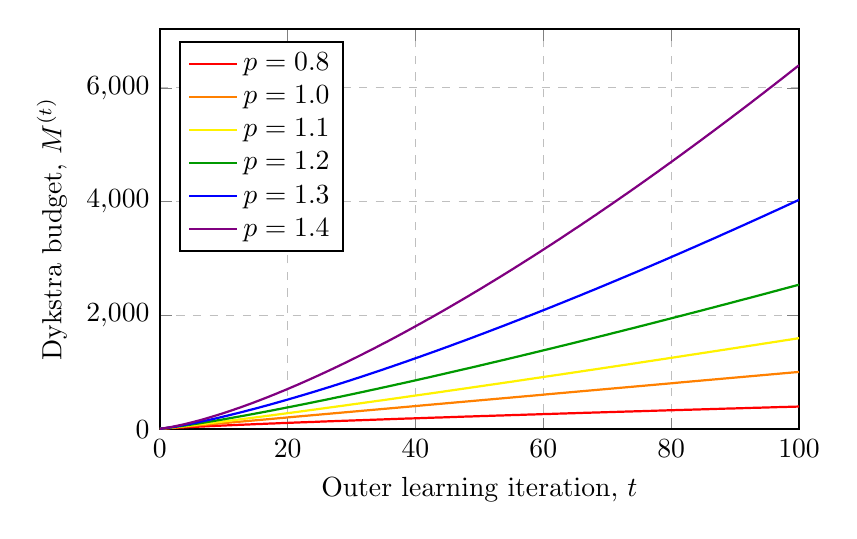
\begin{tikzpicture}
        \begin{axis}[
            width=0.8\textwidth,
            height=0.55\textwidth,
            xlabel={Outer learning iteration, $t$},
            ylabel={Dykstra budget, $M^{(t)}$},
            xmin=0, xmax=100,
            ymin=0,
            grid=major,
            grid style={dashed, gray!50},
            legend pos=north west,
            legend cell align={left},
            thick
        ]

        \addplot[domain=0:100, samples=200, color=red] {floor(10*(x+1)^0.8)};
        \addlegendentry{$p = 0.8$}
        
        \addplot[domain=0:100, samples=200, color=orange] {floor(10*(x+1)^1.0)};
        \addlegendentry{$p = 1.0$}
        
        \addplot[domain=0:100, samples=200, color=yellow] {floor(10*(x+1)^1.1)};
        \addlegendentry{$p = 1.1$}
        
        \addplot[domain=0:100, samples=200, color=green!60!black] {floor(10*(x+1)^1.2)};
        \addlegendentry{$p = 1.2$}
        
        \addplot[domain=0:100, samples=200, color=blue] {floor(10*(x+1)^1.3)};
        \addlegendentry{$p = 1.3$}
        
        \addplot[domain=0:100, samples=200, color=violet] {floor(10*(x+1)^1.4)};
        \addlegendentry{$p = 1.4$}
        
        \end{axis}
    \end{tikzpicture}
    \caption{Dynamic inner Dykstra iteration budget over the outer learning iterations.}
    \label{fig:dynamic_iteration_budget}
\end{figure}

The selection of the scaling exponent $p$ defines distinct computational regimes that must correspond to the convergence rate of the underlying Dykstra projection. When the constraint geometries are poorly conditioned, characterised by sharp geometric angles between intersecting half-spaces, the Dykstra iterates converge slowly to the true projection. In these scenarios, a super-linear exponent ($p > 1$) is required to ensure the dynamic budget outpaces the slow convergence, thereby guaranteeing asymptotic feasibility. Conversely, if the half-space normals defined by $-A$ are nearly parallel, the inner projection step converges quickly in practice. Under such well-conditioned geometry, the rapid algorithmic convergence removes the need for large iteration ceilings. Deploying a sub-linear exponent ($0 < p < 1$) in this regime yields a concave budget growth that provides a sufficient upper bound to reach the optimum, while strictly bounding the computational expenditure per outer iteration.

\subsection{Inactive constraint removal}
A standard Dykstra cycle iterates through all $n$ half-spaces sequentially. As discussed in Chapter~\ref{ch:dykstra}, the feasible polyhedral intersection $\mathcal{H}$ can be partitioned into an active subset $\mathcal{A}$ and an inactive subset $\bar{\mathcal{A}}$ (see~\eqref{eq:active_inactive_sets}). From~\cite[Lemma~3.1]{DYKSTRAPOLY}, it is established that for indices belonging to $\bar{\mathcal{A}}$, there exists a finite integer iteration threshold beyond which the half-space is permanently inactive. For an inactive half-space $i \in \bar{\mathcal{A}}$, the Euclidean projection acts as the identity mapping, yielding $w^{(m)} = w^{(m-1)}$ and leaving the auxiliary error term strictly zero, $e_i^{(m)} = 0$. Continually evaluating the geometric boundary conditions for these inactive constraints contributes to significant computational overhead. 

To eliminate this overhead, we implement \emph{dynamic half-space removal}. We initialise an active tracking set $\mathcal{I} = \{1, 2, \dots, n\}$. During each projection cycle, if the unconstrained intermediate point satisfies the constraint strictly (i.e., it lies in the interior $\mathrm{int}\,\mathcal{H}_i$) and the corresponding auxiliary error $e_i$ is zero, we deduce the constraint has moved into the inactive set. The index $i$ is subsequently popped from $\mathcal{I}$. For all remaining cycles in the current outer iteration, the Dykstra solver bypasses the removed indices, effectively shrinking the length of a full cycle from $n$ to $|\mathcal{A}|$.

\subsection{Feasibility detection and early termination}
While the schedule in \eqref{eq:dynamic_budget} provides a ceiling for the iteration budget, the sequence of projections will sometimes find a physically valid coefficient vector before hitting the full budget $M^{(t)}$. Forcing the algorithm to exhaust the budget to find the exact Euclidean limit point is computationally wasteful, particularly because the subsequent outer unconstrained step will immediately displace the coefficients. To prevent redundant cycles, we implement a strict feasibility-based early termination criterion. Rather than monitoring the spatial displacement between consecutive iterates, the solver evaluates whether the current coefficient vector strictly satisfies the complete polyhedral intersection $\mathcal{H}$. 

This evaluation is applied at two distinct stages. First, before the projection loop begins, the solver checks the initial unconstrained point $w^\circ$. If the gradient descent step happens to land inside the feasible set (satisfying $-A w^\circ \le -\epsilon_m$), the projection mechanics are bypassed entirely, requiring zero inner iterations. Second, at the conclusion of each full Dykstra cycle, the solver re-evaluates the updated coefficient vector $w$. The moment the coefficients become strictly monotonic across all spatial boundaries, the inner loop terminates and returns the feasible iterate. 

Algorithm~\ref{alg:accelerated_dykstra} summarises the integration of the dynamic budget, constraint pruning, early termination, and the stall fast-forwarding mechanisms derived in Chapter~\ref{ch:dykstra}.

\begin{algorithm}[H]
\caption{Accelerated Inexact Dykstra Projection}
\label{alg:accelerated_dykstra}
\begin{algorithmic}[1]
\State \textbf{Input:} Outer iteration $t$, unconstrained weights $w^\circ \in \mathbb{R}^d$, constraints $-A \in \mathbb{R}^{n \times d}$, tolerances $-\epsilon_m \in \mathbb{R}^n$, base budget $M_{\mathrm{base}}$, scaling exponent $p$
\State $M^{(t)} \gets \lfloor M_{\mathrm{base}} (t+1)^p \rfloor$ \algcomment{Calculate dynamic iteration budget}
\State $w \gets w^\circ$
\State $e_i^{(0)} \gets \mathbf{0}_d \quad \forall i \in \{1, \dots, n\}$ \algcomment{Initialise auxiliary variables}
\State $\mathcal{I} \gets \{1, 2, \dots, n\}$ \algcomment{Initialise active index set}

\For{$m = 0, 1, \dots, M^{(t)}-1$}
    \For{$i \in \mathcal{I}$}
        \State $w \gets \mathrm{FF}(w, -A, -\epsilon_m)$ \algcomment{Stalling fast-forwarding as per Algorithm~\ref{alg:fastforward}}
        \State $w^{(m)} \gets w$
        \State $w \gets \mathcal{P}_{\mathcal{H}_i}(w^{(m)} + e_i^{(m)})$ \algcomment{Project onto individual half-space}
        \State $e_i^{(m+1)} \gets e_i^{(m)} + w^{(m)} - w$ \algcomment{Update auxiliary error}
        
        \If{$w = w^{(m)}$ \textbf{and} $e_i^{(m+1)} = \mathbf{0}_d$}
            \State $\mathcal{I} \gets \mathcal{I} \setminus \{i\}$ \algcomment{Prune inactive half-space}
        \EndIf
    \EndFor
    
    \If{$-A w \le -\epsilon_m$}
        \State \textbf{break} \algcomment{Terminate early on feasibility}
    \EndIf
\EndFor
\State \textbf{Return} $w$
\end{algorithmic}
\end{algorithm}

This algorithm acts as the $\mathrm{Dykstra}(\cdot)$ function called by the master framework in line 14 of Algorithm~\ref{alg:inexact_pgd}.
\section{Summary} \label{sec:optimisation_summary}

This chapter has developed a scalable, inexact projection framework to compute the optimal transport map parameterisation, which is summarised in Algorithms~\ref{alg:inexact_pgd}--\ref{alg:accelerated_dykstra} and complemented by Algorithm~\ref{alg:fastforward} developed in Chapter~\ref{ch:dykstra}. By integrating stochastic gradient evaluation and iterative hard thresholding into an outer projected gradient descent loop, the architecture navigates flat objective landscapes and enforces structural sparsity on the physical parameters. Furthermore, by dynamically scheduling the inner Dykstra iteration budget and implementing feasibility-based early termination criteria, the framework circumvents the computational overhead associated with continuous exact Euclidean projections. 

Together with the theoretical resolution of Dykstra's stalling phenomenon presented in Chapter~\ref{ch:dykstra} and the physical structure of the Knothe-Rosenblatt map derived in Chapter~\ref{ch:optimal_transport}, this computational architecture completes the mathematical foundation of the thesis. The subsequent chapter will demonstrate the efficiency of this unified framework by deploying it on several examples, from addressing the problem of propagating non-linear satellite uncertainty in cislunar space to tracking chaotic systems in geophysical applications.

\chapter{Application to orbital mechanics} \label{ch:numerical_experiments}
% \input{sections/5_1_satellite_uncertainty}
% \input{sections/5_2_reconstructing_shear}
% \input{sections/5_3_performance_scaling}

\chapter{Conclusion and future work} \label{ch:conclusion}
\section{Conclusion} \label{sec:conclusion}

\textcolor{red}{CONCLUSION}

\subsection{Dykstra Conclusion}

We identify several directions for future research. First, extending the analysis from polyhedral sets to broader classes of convex sets would enhance the generality of the results. Second, applying our method to a reformulated linear program in which the optimality conditions are decomposed into a convex and a conic set could provide a benchmark for evaluating the proposed approach. Finally, although we have improved Dykstra's overall convergence properties by eliminating stalling, we have not been able to show that our modified version yields iterates $x_m$ that \emph{monotonically} approach the projection $x^\star$. According to the analysis in~\cite{DYKSTRAPOLY}, the algorithm successively discards sets $\mathcal{H}_i$ for which $x^\star\in\text{int}\,\mathcal{H}_i$, and during these phases, the algorithm can produce iterates that temporarily diverge from $x^\star$. Developing a similar fast-forwarding technique for these non-stalling phases would enable monotonic convergence of the iterates, allow \textit{a priori} bounds on the error $\anynorm{x_m-x^\star}$, and provide deterministic guarantees on solution quality for any fixed iteration budget.

\clearpage
\printbibliography

\clearpage
\appendix

\textcolor{red}{APPENDIX}

\end{document}